% Chapter 2

\chapter{The Experimental Apparatus} % Main chapter title

\label{apparatus} % For referencing the chapter elsewhere, use \ref{Chapter1} 

\lhead{Chapter 2. \emph{The Experimental Apparatus}} % This is for the header on each page - perhaps a shortened title

%----------------------------------------------------------------------------------------

This chapter describes the Large Hadron Collider (LHC)~\cite{LHCmachine} and the Compact Muon Solenoid (CMS)~\cite{CMSdetector} detector which records data from pp and heavy ion collisions and is located at one of the main interaction points along the LHC.  The CMS detector is a general-purpose detector that recorded data from 2010 to 2012 corresponding to 36 $\text{pb}^{-1}$ and 5 $\text{fb}^{-1}$ at $\sqrt{7}$ TeV and 19.6 $\text{fb}^{-1}$ at $\sqrt{8}$ TeV.  Section~\ref{lhcsection} contains details on the design and specifications of the LHC and section~\ref{cmssection} describes the CMS detector, its sub-systems, and a number of upgrades (both completed and planned) that it has undergone.

\section{The Large Hadron Collider}
\label{lhcsection}

The LHC is a two-ring-superconducting-hadron accelerator and collider that sits in the 26.7 km tunnel that was constructed for and housed the Large Electron Positron collider (LEP).  It is capable of delivering pp, lead-lead, and proton-lead collisions.  This section will focus on pp collisions.

\subsection{Design}

In 1994 the proposal to the CERN council to construct the LHC in the existing LEP tunnel was approved.  With the Superconducting Super Collider (SSC) canceled just the year before due to concerns related to rising costs, the ability to use a preexisting tunnel was a significant motivation for construction of the LHC to be located there.  As a result the layout of the LHC was strongly influenced by geometry of the LEP tunnel.

Before reaching the full collision energies, particles in the LHC must go through a series of accelerators in which they are successively brought to higher and higher energies.  This system, composed of an initial linear accelerator and a number of synchrotrons, is called the injection chain and consists of the following systems:

\begin{itemize}
\item The linear accelerators (LINACs) are the first step in the chain.  The LINAC2 accelerator generates the protons at an energy of 50 MeV for injection in to the smallest synchrotron.
\item The Proton Synchrotron Booster (PSB) prepares the protons for injection in to the next step, the Proton Synchrotron (PS).  In it the protons are accelerated to 1.4 GeV.
\item The PS then raises the proton energy to 26 GeV.
\item The last step before injection in to the LHC itself, the Super Proton Synchrotron (SPS) accelerates the proton beams to 450 GeV.
\item Finally, once in the LHC, the proton beams are accelerated to the energies at which they will collide.  In 2010 and 2011 the operating energy here was 3.5 TeV, in 2012 the energy per beam was increased to 4 TeV.  Currently, in 2015, the proton beams circulating in the LHC each possess an energy of 6.5 TeV.
\end{itemize}

These accelerators are depicted in Figure~\ref{figapp:LHCinjection} with their approximate relative sizes and locations.

\begin{figure}[!Hh]
       \centering
       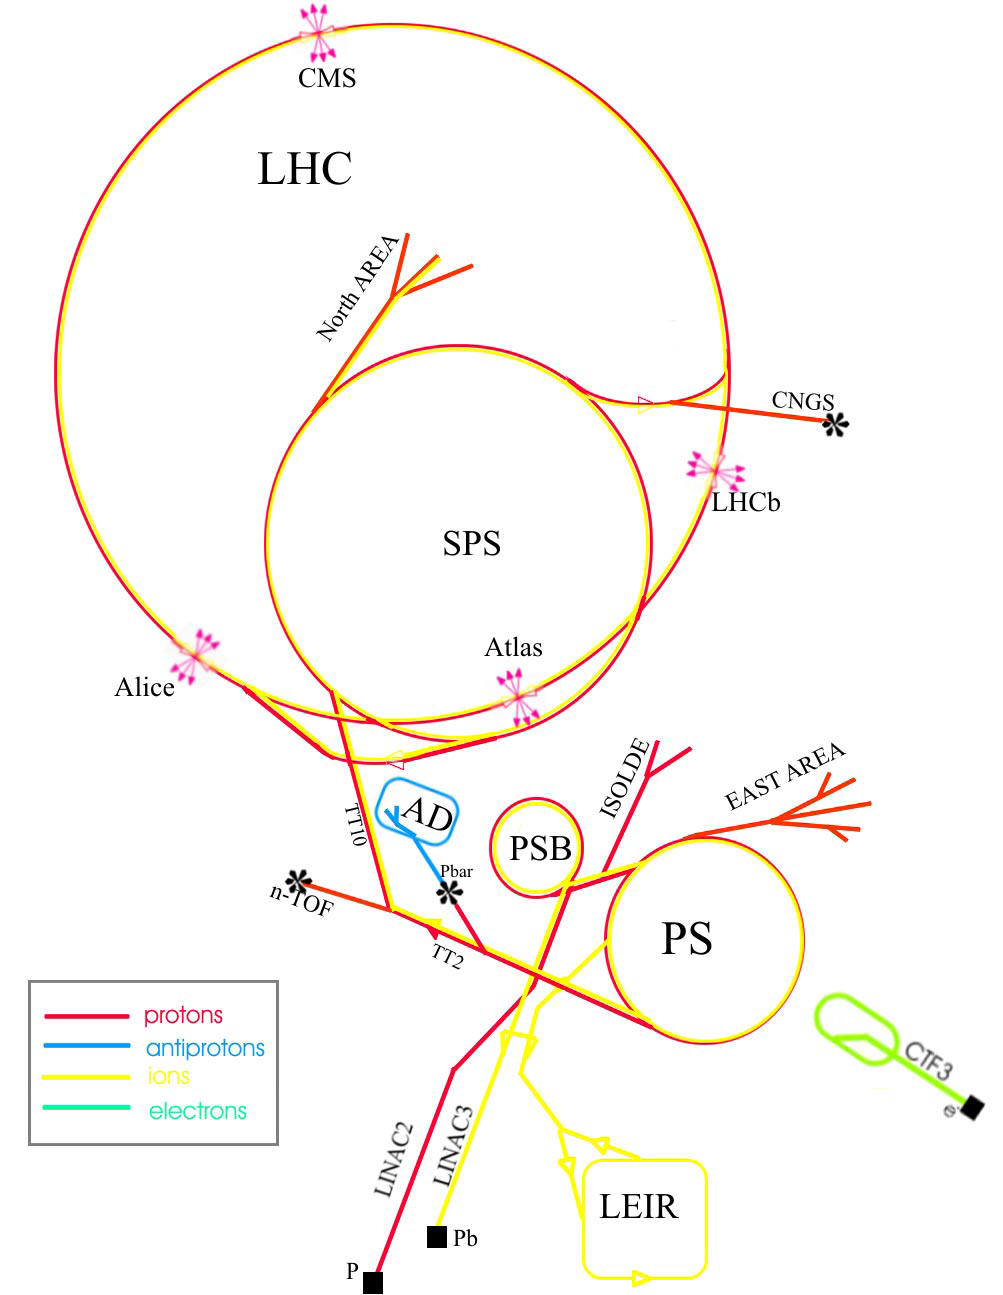
\includegraphics[scale=0.1]{Figures/PSnew.jpg} 
       \caption[Schematic of the LHC injection chain system.]{A schematic of the injection chains of the successive accelerators in to the LHC.  The LINACs at the bottom of the diagram inject the protons or the lead ions which enter the LHC via the PSB, PS, and SPS.  The approximate relative size of each system is shown, as well as relative locations.}
\label{figapp:LHCinjection}
\end{figure}


Once accelerated to these energies the beams are made to collide at four points along the LHC ring.  The LHC has eight arcs and eight straight sections.  Each straight section is 528 m long and can serve as an experimental or insertion point.  Point 1, in the center of the first ``octant'', is the location of the ATLAS (A Toroidal LHC Apparatus) experiment, while CMS is located across the LHC ring at Point 5.  Points 2 and 8 are the locations of the ALICE (A Large Ion Collider Experiment) and LHCb (LHC beauty) experiments, as well as the injection points for Beam 1 and Beam 2 (the main colliding beams used in the LHC).  These 4 points are where the beams cross at interaction points (IPs), where the $\beta$ function is low and the beams are squeezed.  The remaining 4 octants do not contain IPs, rather Points 3 and 7 contain collimations systems, Point 4 contains an RF system, and Point 6 is the location of the beam dump system.  This consists of a combination of horizontally deflecting fast-pulsed magnets and vertically deflecting double steel septum magnets that serve to vertically extract both beams~\cite{LHCmachine}.  This layout is depicted in Figure~\ref{figapp:LHClayout}.



\begin{figure}[!Hh]
       \centering
       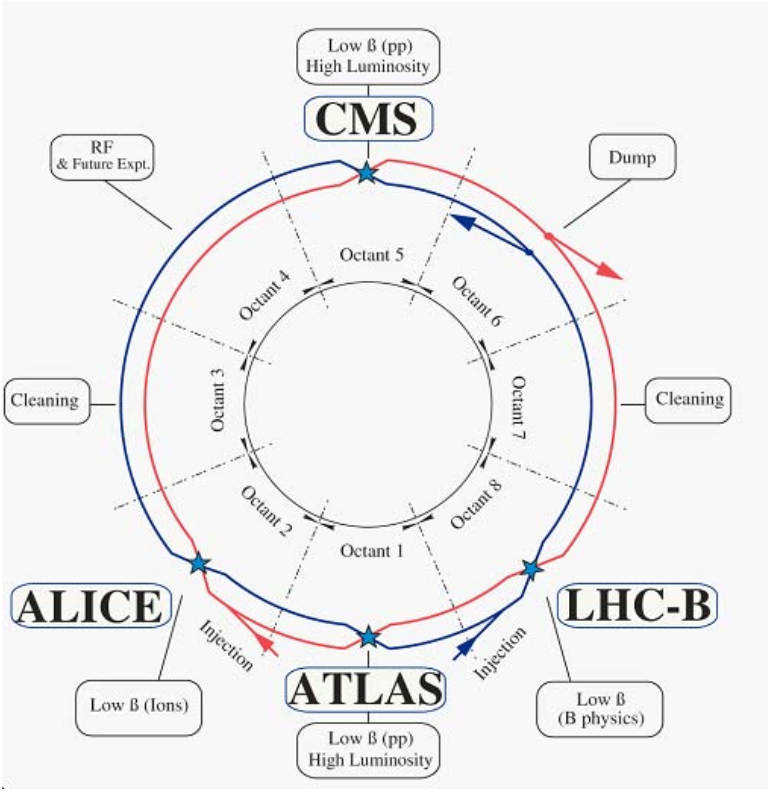
\includegraphics[scale=0.5]{Figures/LHClayout.png} 
       \caption[Schematic of the LHC layout.]{A schematic of the layout of the LHC.  Points 1, 2, 5, and 8 are the locations of the 4 experiments conducted at the LHC~\cite{LHCmachine}.}
\label{figapp:LHClayout}
\end{figure}

Each of the eight arcs that compose the majority of the LHC's 26.7 km is composed of 23 cells, each 106.9 m long, making each arc approximately 2.5 km in length.  Each arc cell itself is composed of two half cells each containing a cold mass (6.63 m long cryostat), a short straight section (SSS), and three dipole magnets 14.3 m in length.  This comes to a total of 1104 main dipoles in use in the LHC ring straight sections and with 128 more in use in the straight regions the LHC contains 1232 dipole magnets in total.  Each dipole is held to a temperature of 1.9 K in operation and provides a magnetic field (at the 7 TeV beam energy) of 8.33 T.  At this operating level the current through the dipole magnets is 11.85 kA.  The layout of the dipole magnets is given in Figure~\ref{figapp:LHCdipole}.  The SSSs contain the main quadrupole magnets and a variety of magnets such as skew quadrupole correctors, sextupole-dipole correctors, tuning quadrupoles, and octupoles.  


\begin{figure}[!Hh]
       \centering
       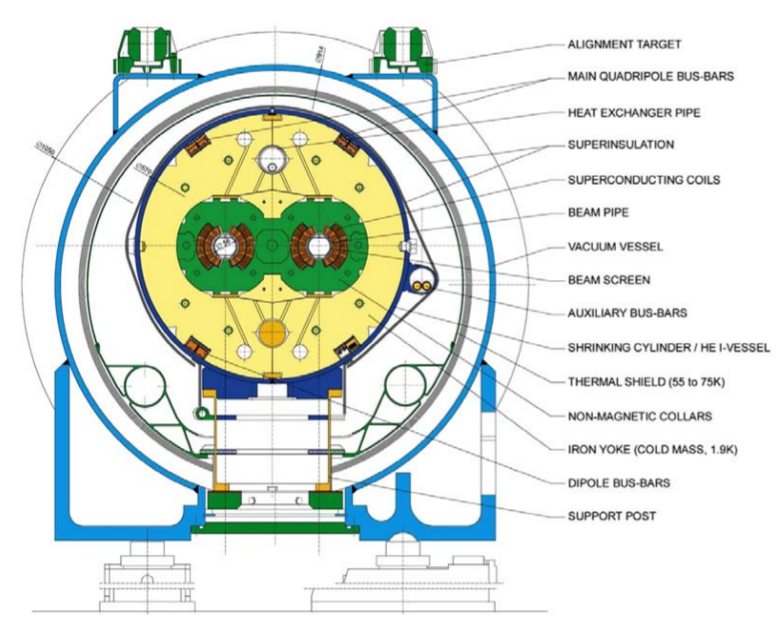
\includegraphics[scale=0.5]{Figures/LHCdipole.png} 
       \caption[Diagram of an LHC cryodipole.]{Diagram of a cross section of an LHC ``cryodipole'': the combined assembly housing the superconducting dipole magnets and the cold mass~\cite{LHCmachine}.}
\label{figapp:LHCdipole}
\end{figure}


\subsection{Specifications and parameters}

The aim of the LHC being to reveal physics beyond the standard model, not only must the beam energy be high to reveal processes suppressed in nature due to kinematics, but also integrated luminosity is a limiting variable for statistically limited searches.  The integrated luminosity over a period of time, $T$, is given by:

\begin{equation}
\mathcal{L} = \int_{T}{\text{L} dt}
\label{eq:IntLuminosity}
\end{equation}

where L is the luminosity and is measured in number of collisions the LHC can produce per unit area per unit time (machine luminosity).  Given a particular physics process of interest, $P$, the number of expected events for such a process over a period of time $T$ is:

\begin{equation}
N_{event}(P) = \int_{T}{\text{L} \sigma_{event}(P) dt}
\label{eq:NumEvents}
\end{equation}

where $\sigma_{event}(P)$ is the cross section for the event of the process in question and depends on the the energy in the event and the model in question.  The instantaneous luminosity, $L$, depends only on the beam parameters and is given by the expression:


\begin{equation}
L = \frac{N^2_b n_b f_{rev} \gamma_r}{4 \pi \epsilon_n \beta^*} F
\label{eq:InstLuminosity}
\end{equation}

where $N_b$ is the number of particles per bunch, $n_b$ is the number of bunches per beam, $f_{rev}$ is the revolution frequency, $\gamma_r$ is the relativistic gamma factor, $\epsilon_n$ is the normalized transverse beam emittance, $\beta^*$ is the beam beta function at the collision point, and F is the geometric luminosity reduction factor due to the crossing angle at the IP.  The value for F is given by the following expression:


\begin{equation}
F = \left(1+\left(\frac{\theta_c \sigma_z}{2 \sigma^*}\right)^2\right)^{-1/2}
\label{eq:BeamF}
\end{equation}

where $\theta_c$ is the full crossing angle at the IP, $\sigma_z$ is the RMS bunch length, and $\sigma^*$ is the transverse RMS beam size at the IP.  This assumes round beams, with $\sigma_z \ll \beta$, as well as assuming equal beam parameters for both beams.  

The discovery of rare processes at the LHC relies upon high energies, high instantaneous luminosities, and significant run times.  The maximum particle density per bunch is limited by nonlinear beam-beam interactions that occur when bunches from the two beams collide with each other.  This beam-beam interaction is measured by the linear tune shift which is given by:



\begin{equation}
\xi = \frac{N_b r_p}{4 \pi \epsilon_n}
\label{eq:LinearTuneShift}
\end{equation}

where $r_p$ is the classical proton radius, $r_p = e^2 / (4 \pi \epsilon_0 m_p c^2)$.  Previous experience with hadron colliders has indicated that the total linear tune shift including all IPs should not exceed 0.015~\cite{LHCmachine}.  The LHC runs pp collisions in 3 experiments simultaneously, so parameters at the LHC must satisfy $\xi < 0.005$.


The LHC beam energy was 3.5 TeV per beam in 2010 and 2011, increasing to 4 TeV in 2012.  The peak instantaneous luminosity during these run periods was a fraction of the nominal value, starting at 2\% in 2010 and increasing to 35\% in 2011 and 77\% in 2012.  The running parameters for 2012 and nominal design conditions are given in Table~\ref{tab:LHCparams}.  Achieving 77\% of nominal with half the nominal number of bunch was achieved partially due to the excellent beam quality delivered by the injectors, yielding an above-nominal number of protons per bunch.  Challenges have arisen, unique to operating complex systems and electronics in the LHC environment.  Occasional beam dumps can be caused by Unidentified Falling Objects (UFOs), and Single Event Effects (SEEs) caused by beam induced radiation to tunnel electronics was a significant source of inefficiency at the onset of the 2011 run~\cite{LHCstatus}.  As the 2015 run is ongoing, with the higher beam energy of 6.5 TeV, UFOs pose an increased challenge to LHC operation.  Looking forward, a series of long shutdowns will prepare the LHC for the High Luminosity LHC program, for which CMS is preparing upgrades to handle and take advantage of the increased rate.  


\begin{table}[!Hhtbp]
\centering
\begin{tabular}{llcc}
\hline
{} & {Parameter}  & {LHC Design Value} &{Achieved in 2012 run}\\
\hline
\hline
{$N_b$} & {Number of particles per bunch} & {$1.15 \times 10^{11}$} &{$1.6-.17 \times 10^{11}$}\\
{$n_b$} & {Number of bunches per beam} & {2808} &{1374}\\
{$f_{rev}$} & {Revolution frequency} & {11.25 kHz} & {11.25 kHz}\\
{$\gamma_r$} & {Relativistic gamma factor} & {7461} &{4263}\\
{$\epsilon_n$} & {Transverse beam emittance} & {$3.75 \mu \text{m}$} &{$2.5 \mu \text{m}$}\\
{$\beta^*$} & {Beta function at IP} & {0.55} &{0.6}\\
{$\theta_c$} & {Crossing angle at IP} & {$285 \mu \text{rad}$} &{$290 \mu \text{rad}$}\\
{$\sigma_z$} & {RMS bunch length} & {7.55 cm} &{9 cm}\\
{$\sigma^*$} & {Transverse RMS beam size at IP} & {$16.6 \mu \text{m}$} &{$19 \mu \text{m}$}\\
{$L$} & {Peak instantaneous luminosity} & {$1 \times 10^{34}$} &{$7.7 \times 10^{33}$}\\
{} & {Bunch spacing} & {25 ns} &{50 ns}\\
{} & {Stored beam energy} & {362 MJ} &{~140 MJ}\\
{} & {Beam energy} & {7 TeV} &{4 TeV}\\
\hline
\end{tabular}
\\
\caption[LHC running parameters, designed and achieved in 2012.]{The targeted design values for the running parameters of the LHC and the values achieved in the 2012 run~\cite{LHCstatus}.}
\label{tab:LHCparams}
\end{table}


\section{The Compact Muon Solenoid}
\label{cmssection}

The IP at Point 5 is the location of the Compact Muon Solenoid (CMS), a general purpose detector used for a variety of higgs and exotic searches and SM measurements.  In 2012, an integrated luminosity of 21.79 $\text{fb}^{-1}$ was recorded by the CMS detector, the integrated luminosity and peak daily luminosities and shown in Figure~\ref{figapp:CMSLumi2012}.  On ~\textcolor{red}{FIXME: Insert date and lumi plots here for 2015 progress} it has recorded a luminosity of ~\textcolor{red}{X} $\text{fb}^{-1}$, shown in Figure~\ref{figapp:CMSLumi2015}.This section describes the CMS detector and its subsystems.  Section\label{cscelectronics} goes in to greater detail regarding the electronics used in the endcap muon subsystem as the author of this thesis was responsible for work on upgrading a component of those systems.  



\begin{figure}[!Hh]
       \centering
       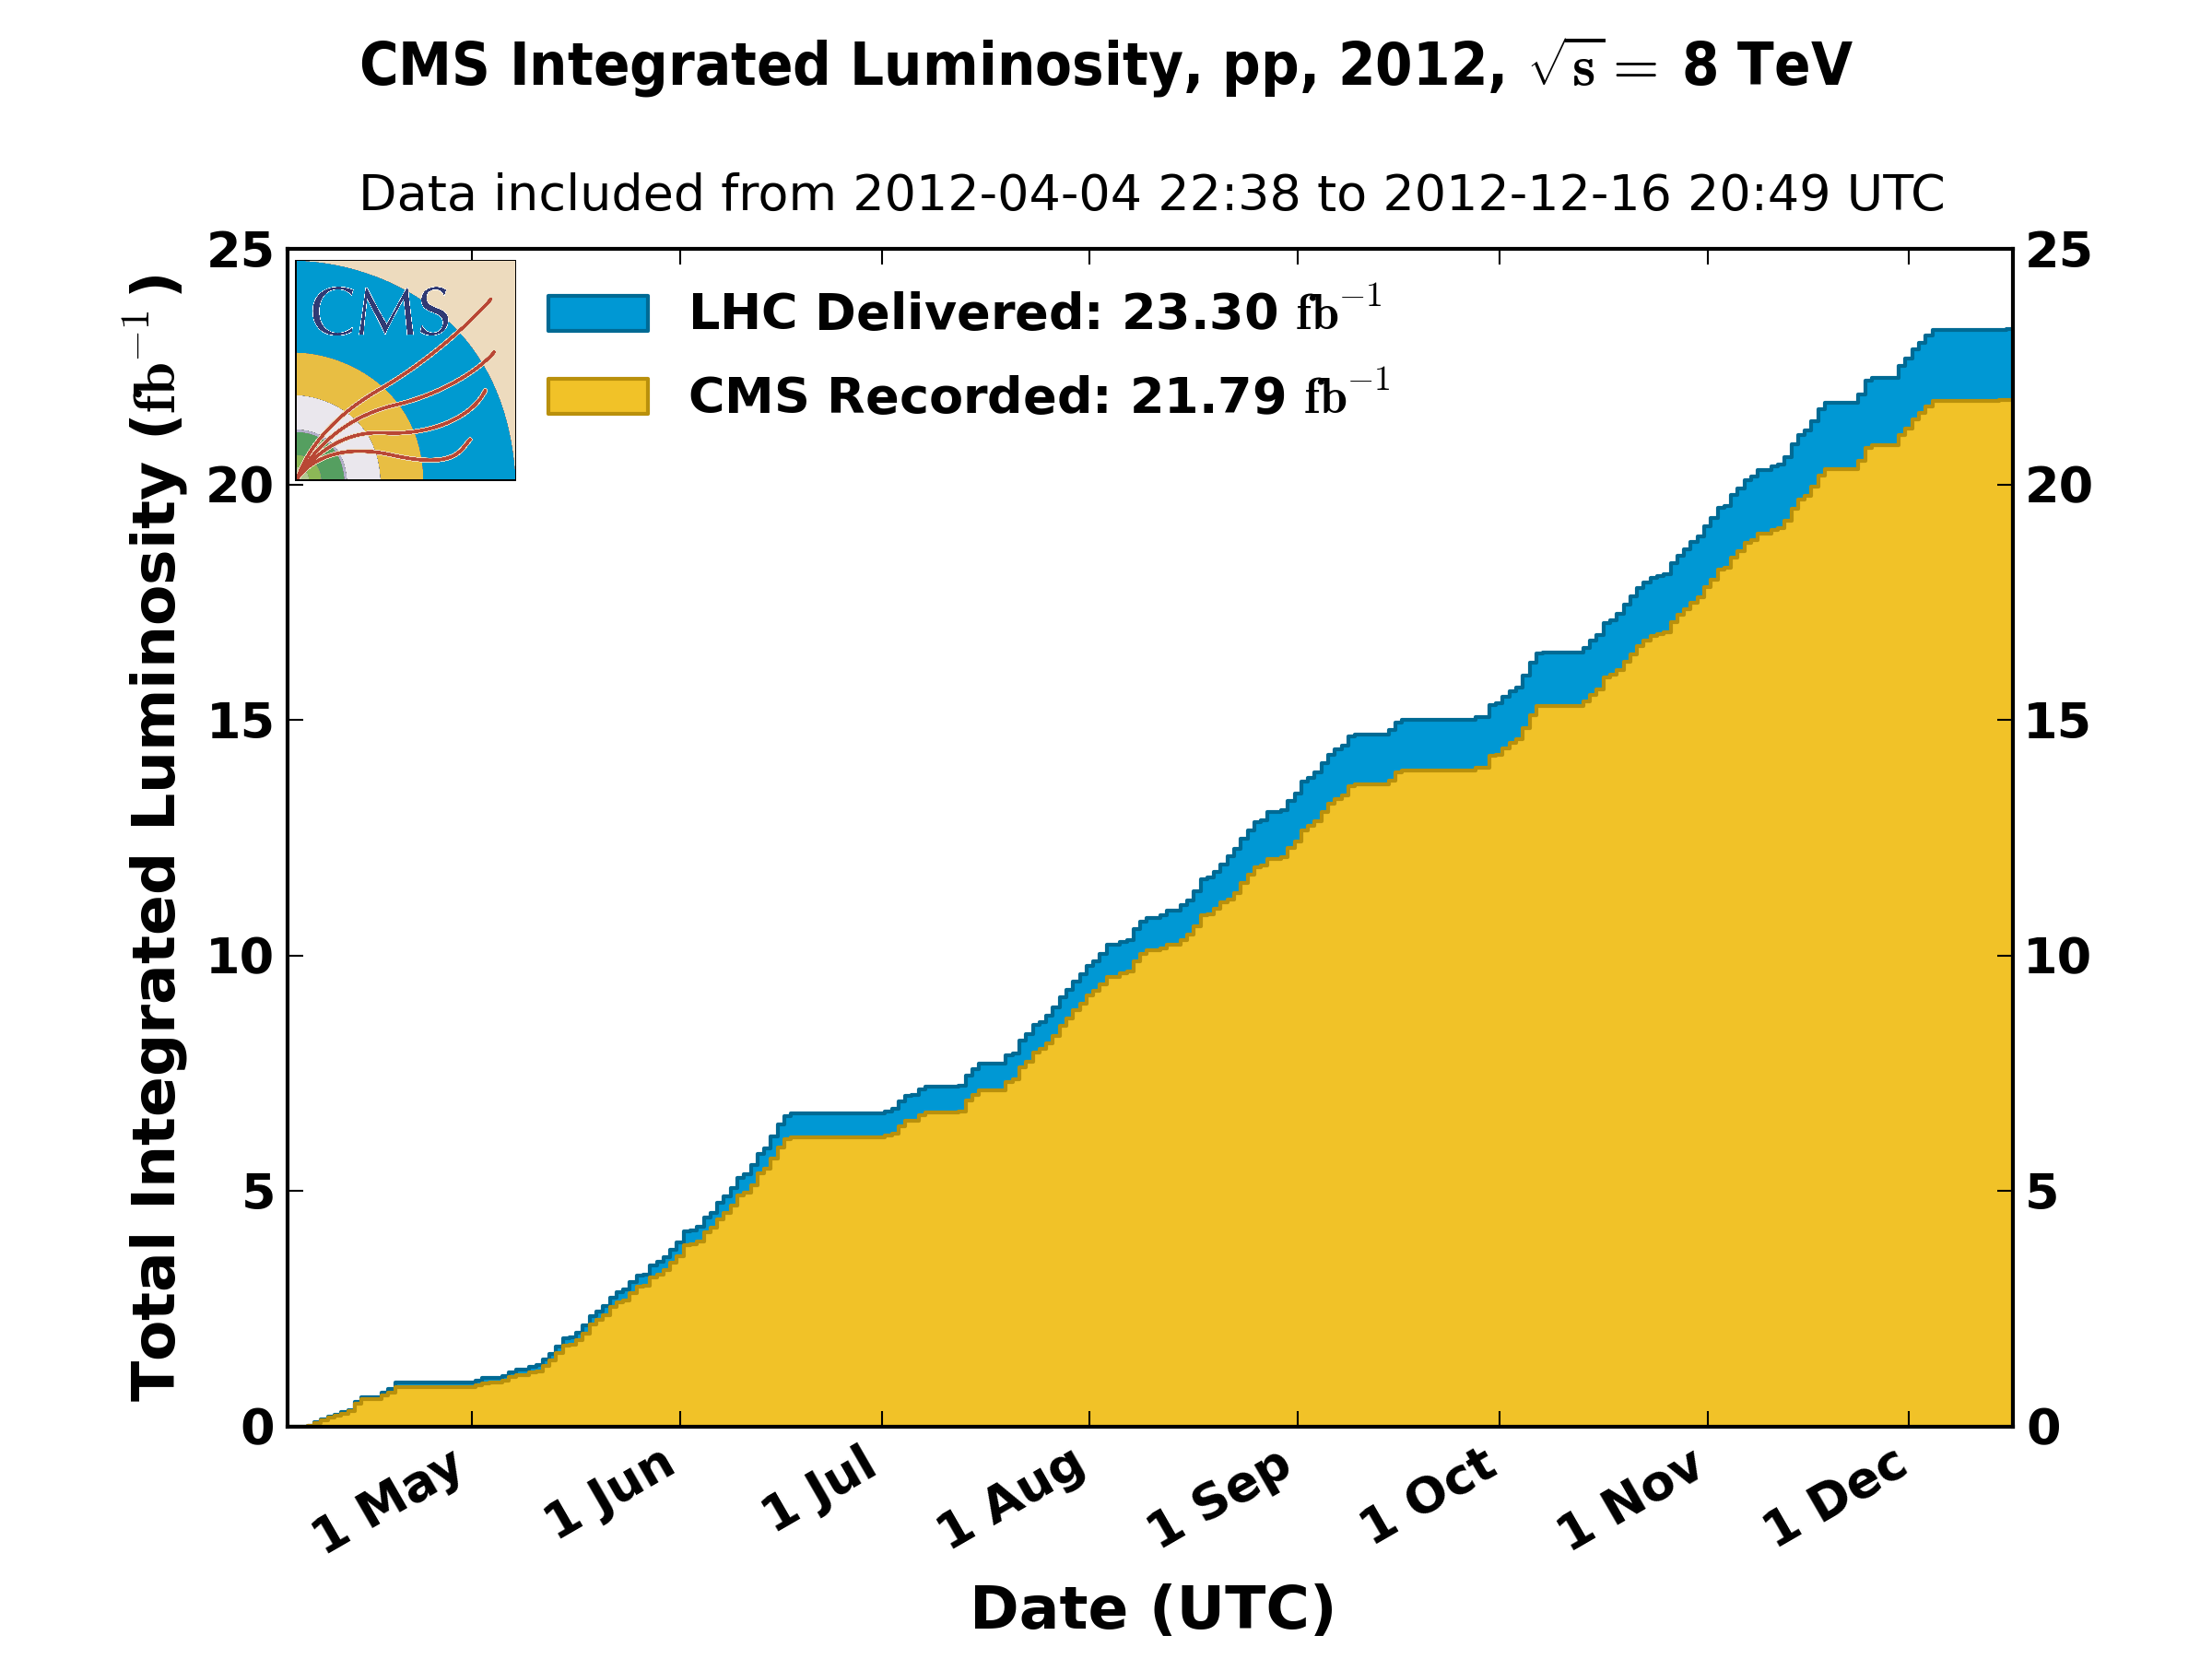
\includegraphics[scale=0.5]{Figures/int_lumi_per_day_cumulative_pp_2012.png} \\
       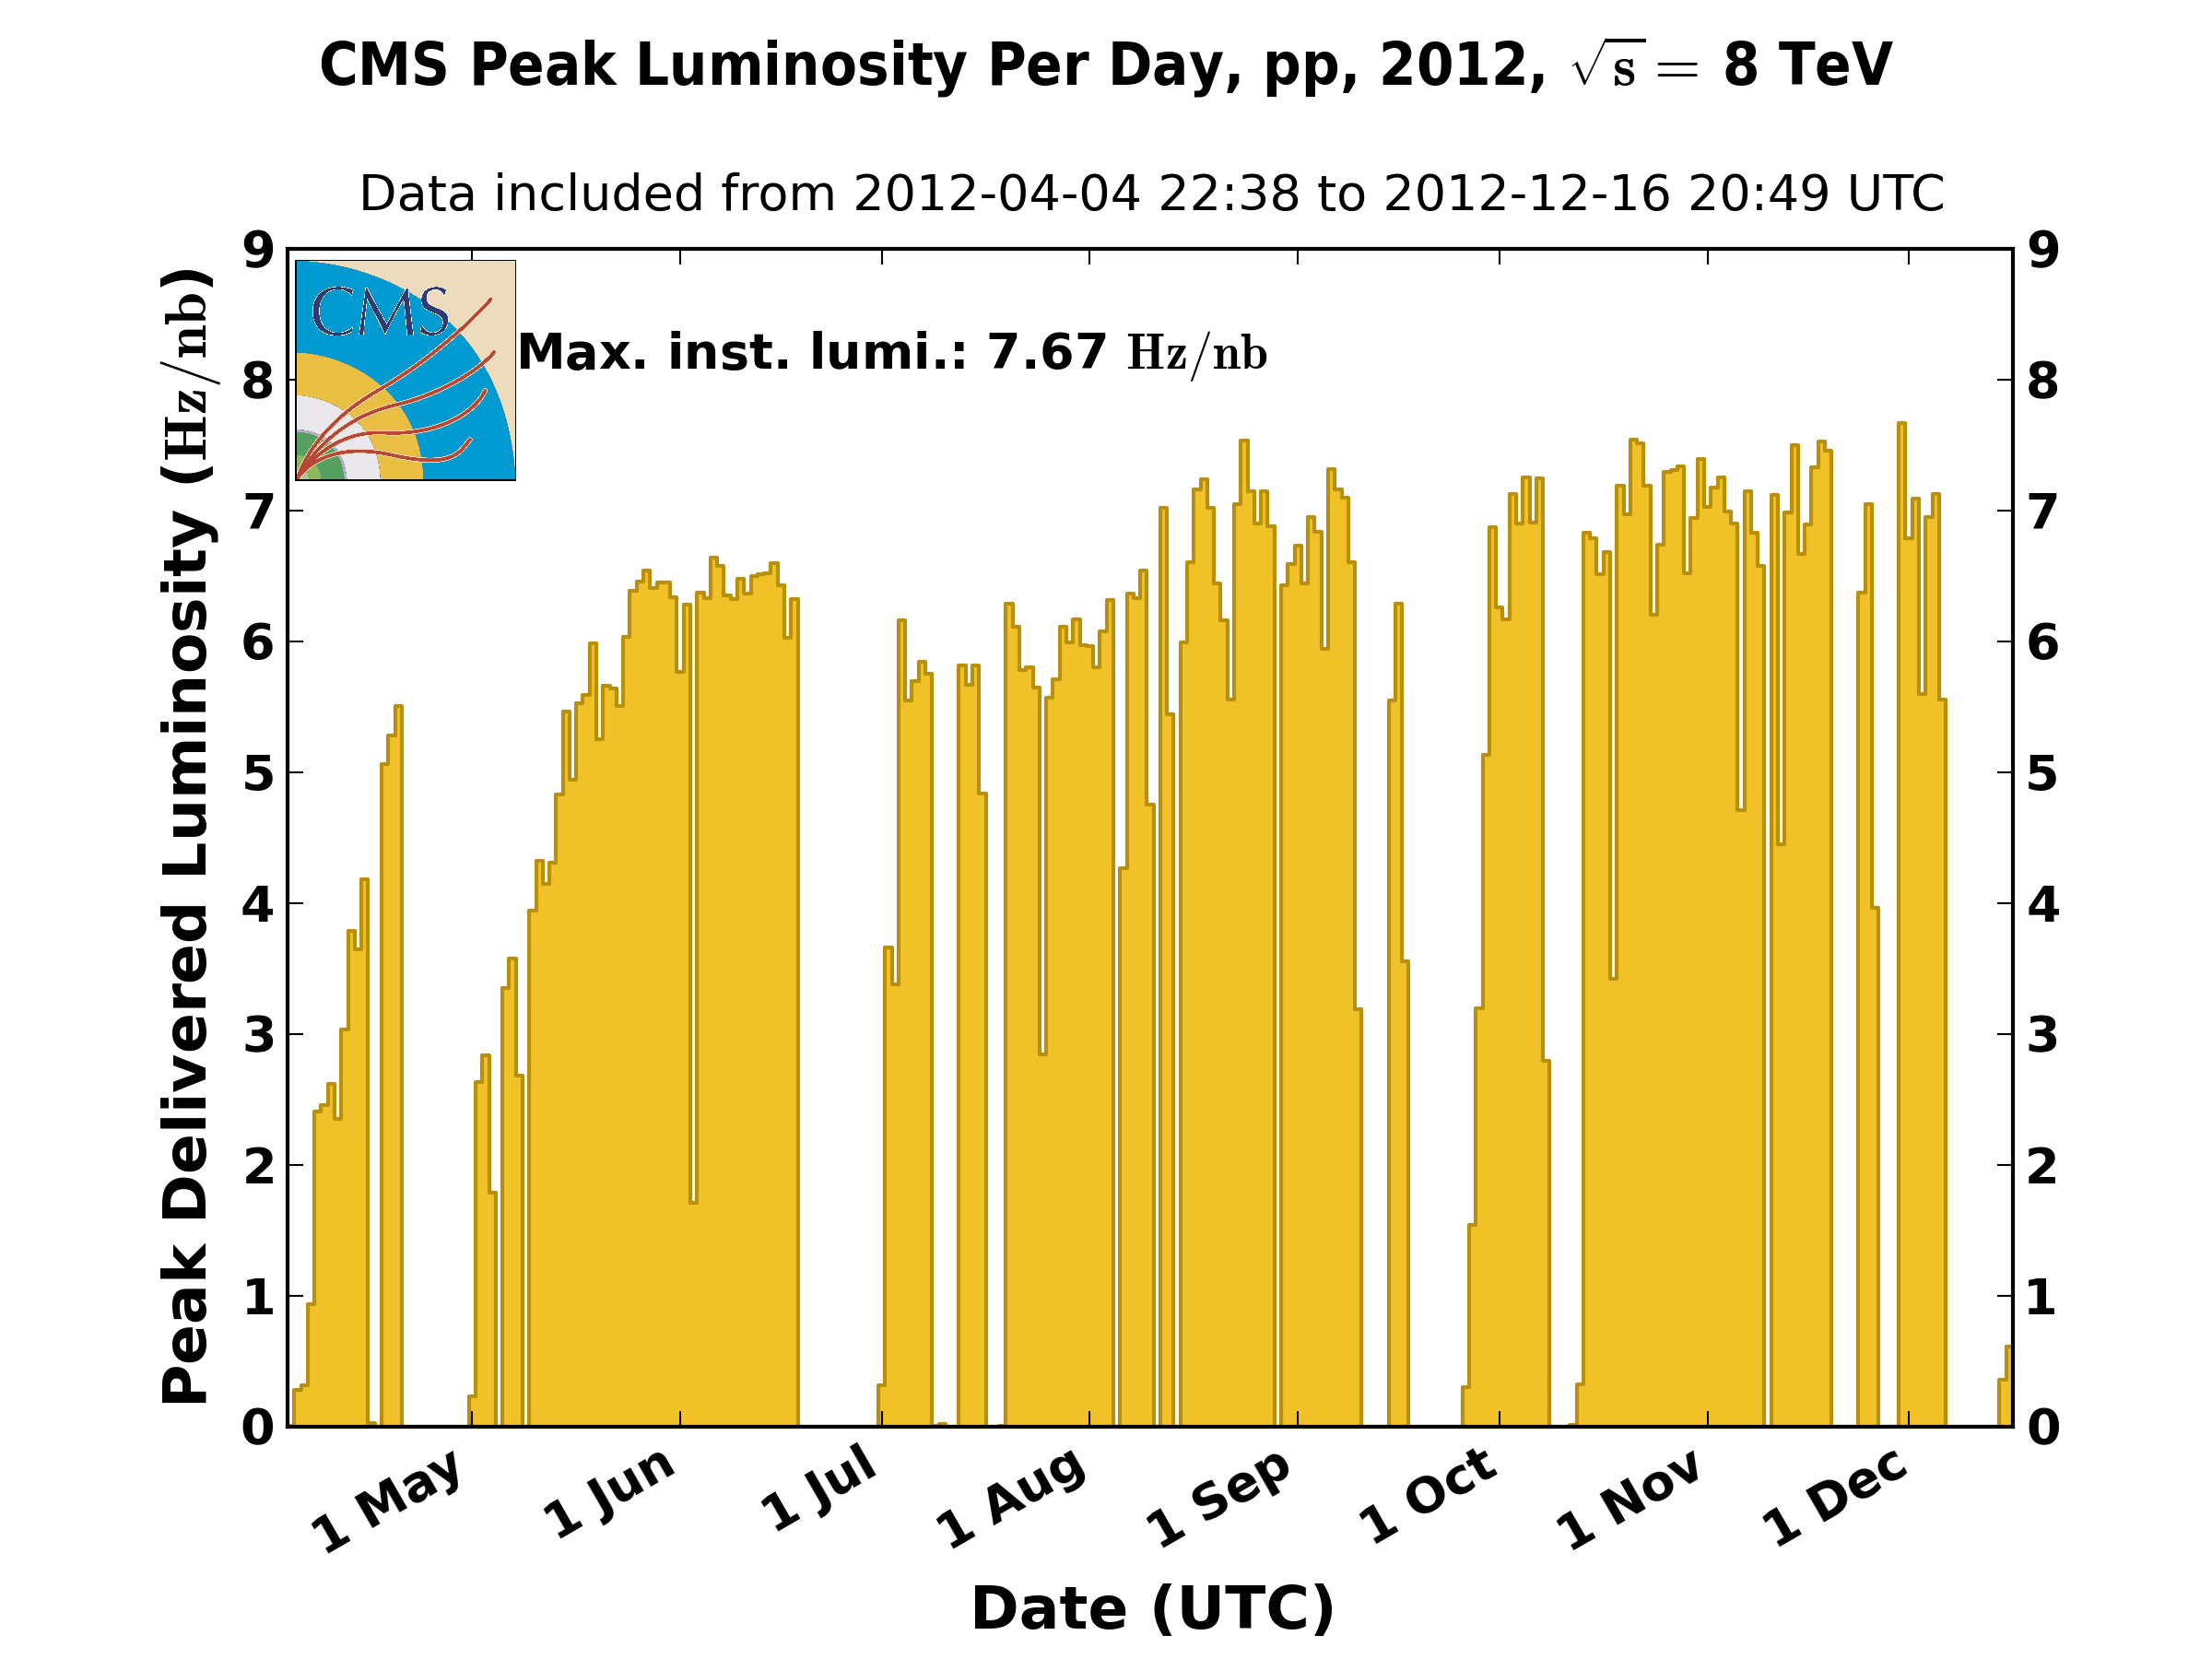
\includegraphics[scale=0.5]{Figures/peak_lumi_per_day_pp_2012.png} 
       \caption[Integrated and peak luminosity per day recorded by CMS in 2012.]{The integrated luminosity (top) delivered to and recorded by the CMS detector and the peak instantaneous luminosity (bottom) in 2012.}
\label{figapp:CMSLumi2012}
\end{figure}


\begin{figure}[!Hh]
       \centering
       \caption[Integrated and peak luminosity per day recorded by CMS in 2015.]{\textcolor{red}{FIXME: Add plots} The integrated luminosity (top) delivered to and recorded by the CMS detector and the peak instantaneous luminosity (bottom) in 2015 by \textcolor{red}{FIXME: Insert dates}.}
\label{figapp:CMSLumi2015}
\end{figure}



\subsection{Overview of the Detector}

The CMS detector is located at Point 5 on the LHC ring, approximately 100 m underground near the French village of Cessy, between Lake Geneva and the Jura mountain range.  It is designed to operate with pp collisions at $\sqrt{s} = 14$ TeV and a design luminosity of $10^{34}\text{ cm}^{-2}\text{s}^{-1}$.  With an expected proton-proton cross section of 100 mb at that design energy the event rate will be approximately $10^9$ inelastic events/s.  Computing limitations allow for approximately 100 events/s for storage and subsequent analysis so the online selection process (called the ``trigger'', discussed in Section~\ref{trigger}) must reduce this very large rate.  

The bunching of protons (within one bunch) and the short time between bunches, 25ns in 2015 and 50ns in 2012, result in the phenomeon called pileup in which multiple inelastic collisions are present in a single event.  The average number of collisions per bunch crossing measured in 2012 was 21, and in 2015 this value rose to \textcolor{red}{FIXME: put value}.  These so called pileup-distributions are shown in Figure~\ref{figapp:CMSpileup}.



\begin{figure}[!Hh]
       \centering
       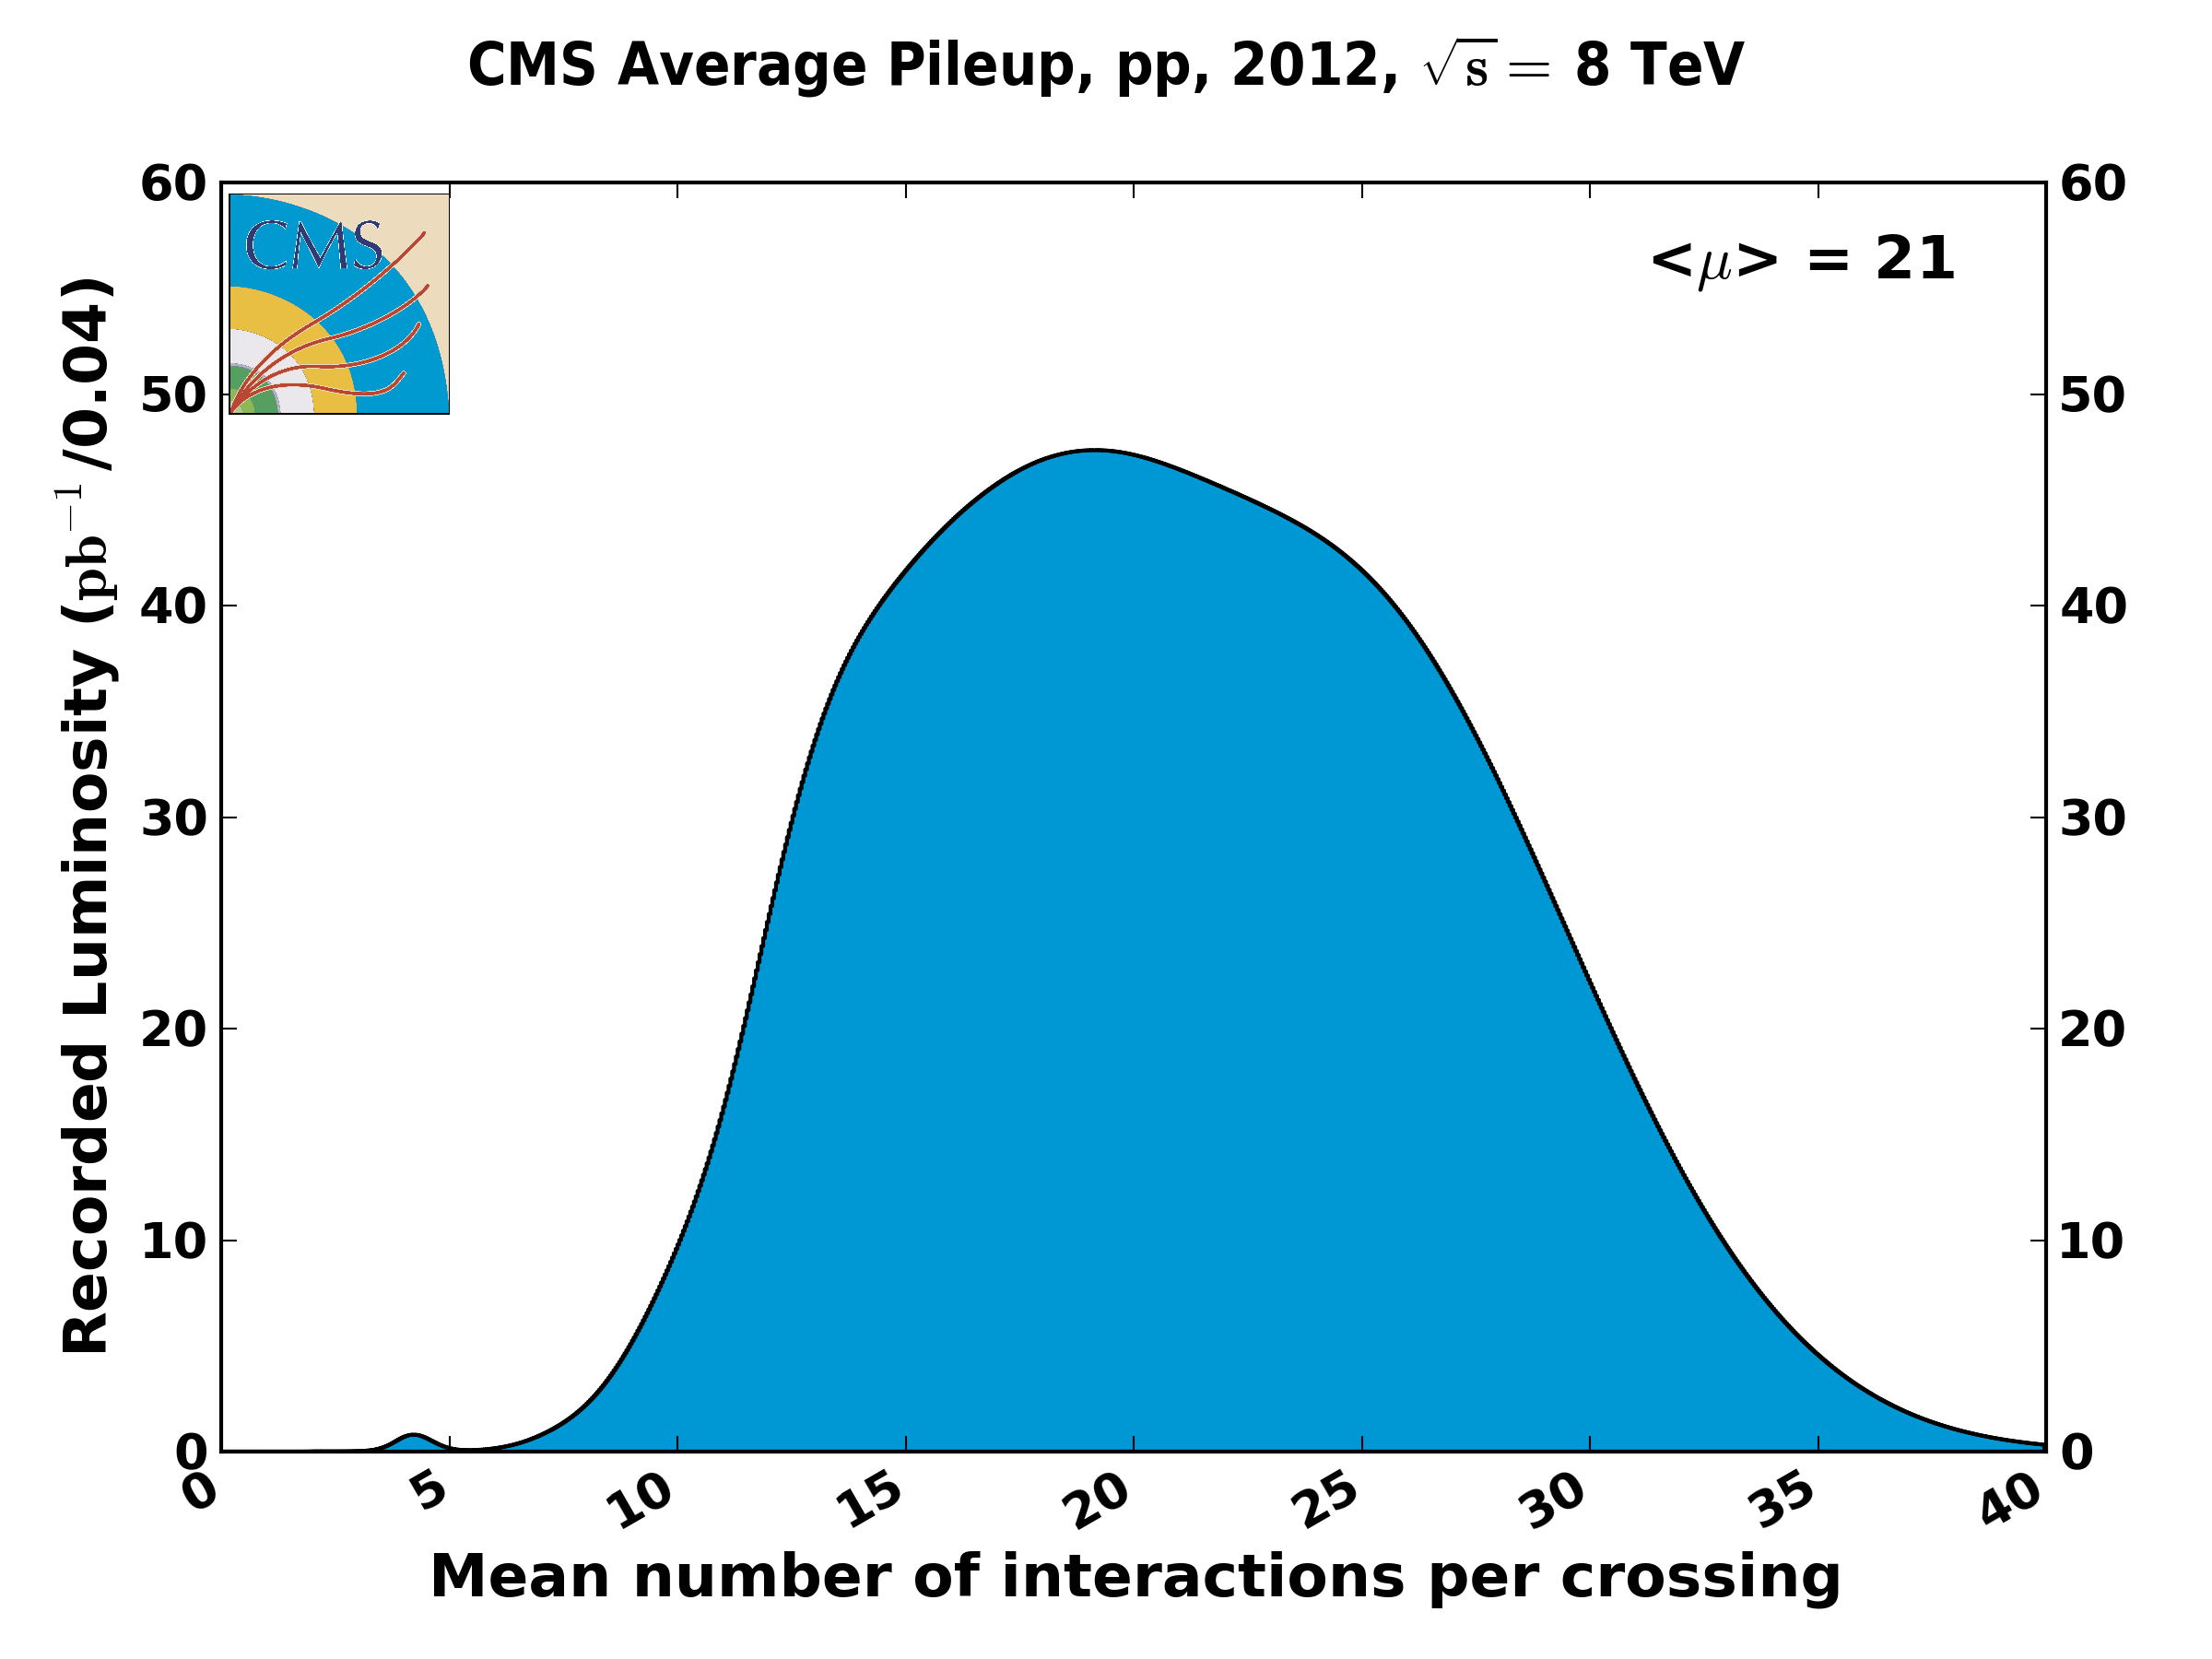
\includegraphics[scale=0.5]{Figures/pileup_pp_2012.png} \\
       \caption[Distribution of number of collisions per bunch crossing in 2012 and 2015.]{\textcolor{red}{FIXME: Add 2015 plot} The distribution of the number of interactions per event measured in 2012 (top) and 2015 (bottom).}
\label{figapp:CMSpileup}
\end{figure}

This results in a significant challenge to avoid confusing products from different interactions in the same collision, especially when response times from subdetectors can exceed the time between bunch crossings.  This effect is reduced in the CMS detector through the use of high-granulaty subdetectors with good time resolution that can achieve low occupancy.  This necessitates a very large number of detector channels, resulting in millions of total detector electronic channels that require good synchronization.  This provides the ability to determine which particles correspond to which event and which collision vertex within the event, and thus correspondingly the ability to accurately reconstruct the charges and momenta of the particles.  

The overall detector requirements for CMS are as follows:

\begin{itemize}

\item Muon systems:
  \begin{itemize}
  \item Good muon identification and momentum resolution for a wide range of momenta and angles
  \item Dimuon mass resolution of approximately one percent at 100 GeV (near the mass of the Z boson)
  \item Near perfect charge determination for muons with momenta less than 1 TeV
  \end{itemize}
\item Electromagnetic calorimeter:
  \begin{itemize}
  \item Good electromagnetic energy resolution
  \item Diphoton and Dielectron mass resolution of approximately one percent at 100 GeV
  \item Rejection of $\pi^0$ decays
  \item Efficient photon and lepton isolation at high luminosities
  \item Wide geometric coverage
  \end{itemize}
\item Inner Tracker:
  \begin{itemize}
  \item Good charged-particle momentum resolution and reconstruction efficiency
  \item Efficient triggering and offline tagging for $\tau$ leptons and jets from $b$-quark decays
  \end{itemize}
  
\item Hadronic calorimeter:
  \begin{itemize}
  \item Good missing-transverse-energy and dijet-mass resolution
  \item Large and hermetic geometric coverage and fine lateral segmentation (enabling the above point)
  \end{itemize}
\end{itemize}

The layout of the subsystems of CMS is shown in Figure~\ref{figapp:CMSlayout}.  Each is described in detail in sections \ref{solenoid} through \ref{muons}.



\begin{figure}[!Hh]
       \centering
       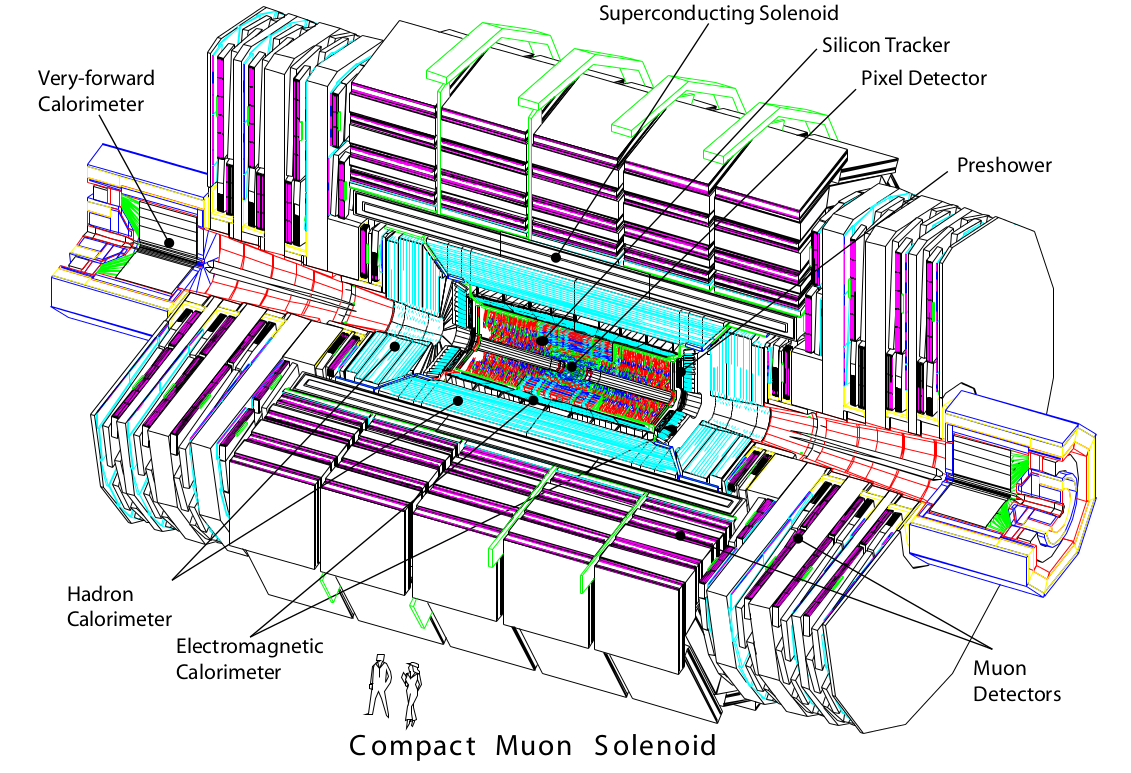
\includegraphics[scale=0.4]{Figures/CMSlayout.png} \\
       \caption[The basic layout of the CMS detector.]{A cutout diagram of the subsystems of the CMS detector, to scale.  The locations of the Solenoid magnet, Calorimeters, Trackers, and Muon Detectors are shown.  Figures of two people standing by the detector are given for a sense of size.}
\label{figapp:CMSlayout}
\end{figure}




\subsection{Conventions and Coordinates}

The convention for describing the geometry of the CMS detector is a right-handed coordinate system, defined with the origin at the nominal IP.  The z-axis points along the beam axis towards the Jura mountains from Point 5.  The y-axis points vertically upward and the x-axis points radially inward to the center of the LHC circle.  Thus the polar angle $\theta$ is taken from the z-axis and the azimuthal angle $\phi$ is measured from the x-axis in the x-y plane.  

Traditionally in collider physics the polar angle $\theta$ is not used, rather the psuedorapidity, $\eta$, is used.  Pseudorapidity is an approximation of the quantity called rapidity, $\varphi$, which is related to an object's speed.  Unlike speeds, at relativistic velocities rapidity is an additive quantity and the difference in rapidity between two particles ejected by a collision is invariant under Lorentz transfomations along the z-axis.  Also, production of particles tends to be close to uniform as a function of $\varphi$.  The rapidity, $\varphi$, is related to the Lorentz $\gamma$-factor as well as energy and momentum of a particle and is given by the expression:



\begin{equation}
\varphi = \cosh^{-1}(\gamma) = \tanh^{-1}\left(\frac{|\bold{p}|c}{E}\right) = \frac{1}{2}\ln\left( \frac{E+|\bold{p}|c}{E-|\bold{p}|c}\right).
\label{eq:rapidity_phi}
\end{equation}


Typically in colliders a version of the rapidity, y, is used that is defined only on the z-axis with respect to longitudinal momentum:

\begin{equation}
y \equiv  \frac{1}{2}\ln\left( \frac{E+p_Lc}{E-p_Lc}\right).
\label{eq:rapidity_y}
\end{equation}


In the limit where the particle's mass is negligible or where the particle is travelling close to the speed of light (applicable in the case of particles coming from collisions in the LHC) the rapidity is approximated by a simple function of the polar angle, $\theta$.  This value is called the psuedorapidity, $\eta$, and is given by the expression:


\begin{equation}
\eta \equiv  -\ln\left[ \tan\left(\frac{\theta}{2}\right)\right].
\label{eq:pseudorapidity}
\end{equation}

Both precision measurements and searches performed at the CMS experiment use kinematics defined in the transverse plane.  This is due to the fact that momentum in that plane can be determined to a high degree of accuracy and momentum conservation can be applied.  Also, like $\eta$, the transverse momentum ($p_T$) is invariant under longitudinal Lorentz transformations.  Thus $p_T$ and $\eta$ are the main kinematic variables used by most searches, including the search discussed in this thesis.  


\subsection{The Superconducting Solenoid}
\label{solenoid}

The superconducting magnet is designed to reach a field of 4 T in a free bore diameter of 6 m and length of 12.5 m, with a stored energy of 2.6 GJ at the full current.  The flux is returned via a 10,000 ton iron yoke which is comprised of five wheels and two endcaps composed of three disks each.  The solenoid itself has a 6.3 m cold bore and weighs 220 tons.  To achieve a 4 T field a very large number of ampere-turns is required (41.7 MA-turns) and the winding of the solenoid is composed of four layers.  This winding is composed of a stabilised and reinforced niobium-titanium (NbTi) conductor.

The ratio between the stored energy and cold mass of 220 t is very high, 11.6 KJ/kg, which results in a very significant mechanical deformation of 0.15\% during energising.  These values are much higher than other solenoidal detector magnets, a comparison of the stored energy and energy-over-mass ratios of the CMS magnet and other detector magnets is given in Figure~\ref{figapp:CMSstoredenergy}.  The main parameters of the CMS magnet are listed in Table~\ref{tab:CMSmagnetparams}.


\begin{figure}[!Hh]
       \centering
       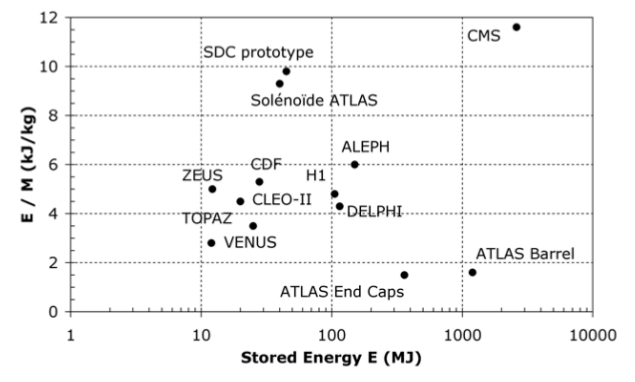
\includegraphics[scale=0.4]{Figures/CMSstoredenergy.png} \\
       \caption[The stored energy of CMS and other detector magnets.]{A comparison of the stored energy and energy-over-mass ratio E/M for CMS and other detector magnets~\cite{CMSdetector}.}
\label{figapp:CMSstoredenergy}
\end{figure}



\begin{table}[!Hhtbp]
\centering
\begin{tabular}{ll}
\hline
\hline
{General parameters} & {}\\
\hline
{Magnetic length} & {12.5 m}\\
{Cold bore diameter} & {6.3 m}\\
{Central magnetic induction} & {4 T}\\
{Total Ampere-turns} & {41.7 MA-turns}\\
{Nominal current} & {19.14 kA}\\
{Inductance} & {14.2 H}\\
{Stored energy} & {2.6 GJ}\\
\hline
\hline
{Cold mass} & {}\\
\hline
{Layout} & {Five modules mechanically and}\\
{} & {electrically coupled}\\
{Radial thickness of cold mass} & {312 mm}\\
{Radiation thickness of cold mass} & {3.9 $X_0$}\\
{Weight of cold mass} & {220 t}\\
{Maximum induction on conductor} & {4.6 T}\\
{Temperature margin w.r.t. operating temperature} & {1.8 K}\\
{Stored energy/unit cold mass} & {11.6 kJ/kg}\\
\hline
\hline
{Iron yoke} & {}\\
\hline
{Outer diameter of the iron flats} & {14 m}\\
{Length of barrel} & {13 m}\\
{Thickness of the iron layers in barrel} & {300, 630, and 630 mm}\\
{Mass of iron in barrel} & {6000 t}\\
{Thickness of iron disks in endcaps} & {250, 600, and 600 mm}\\
{Mass of iron in each endcap} & {2000 t}\\
{Total mass of iron in return yoke} & {10000 t}\\
\hline
\end{tabular}
\\
\caption[Parameters of the CMS magnet.]{The design parameters of the CMS magnet~\cite{CMSdetector}.}
\label{tab:CMSmagnetparams}
\end{table}

The purpose of the magnet is to provide a field that bends muon paths, allowing for precise momentum measurements.  In order to increase the longevity of the magnet, the decision to run it with a field of 3.8 T was made, which degraded the achievable muon momentum resolution by approximately 5\%~\cite{CMSperformance}.  The levels of the magnetic field and structure of the field lines can be seen in Figure~\ref{figapp:CMSfieldlines}, the return of the field the iron yoke is clearly visible.  



\begin{figure}[!Hh]
       \centering
       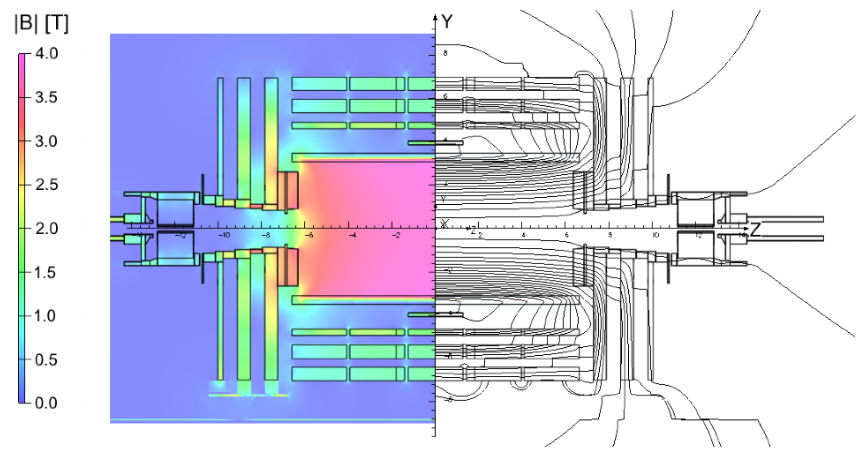
\includegraphics[scale=0.4]{Figures/CMSfieldlines.png} \\
       \caption[The values of the magnetic field and field lines of the CMS magnet in operation.]{A detailed map of the $|B|$ field (left) and the field lines (right) for a longitudinal section of CMS at a magnetic flux density of 3.8 T.  Each field line is an increment in magnetic flux of 6 Wb.~\cite{CMSperformance}.}
\label{figapp:CMSfieldlines}
\end{figure}

\subsection{The Silicon Tracker}
\label{tracker}

The innermost layer of the CMS detector is the inner tracking system, which is composed of an inner pixel tracker with 1440 modules and an outer strip tracker containing 15,148 strip modules.  With a total of approximately 200 $\text{m}^2$ of active silicon area the CMS inner tracker is the largest silicon tracker ever built~\cite{CMSdetector}.  At the LHC design luminosity there is an average of approximately 1000 particles expected per bunch crossing traversing the tracking system, from approximately 20 overlapping proton-proton interactions.  At a radius of 4 cm, the location of the innermost layer of the pixel tracker, this leads to a hit rate density of 1 MHz/$\text{mm}^2$.  In order to meet the resolution requirements the pixel size is $100 \times 150$ $\mu\text{m}^2$ in $r-\phi$ and $z$, respectively, which results in an occupancy of approximately $10^{-4}$ per pixel per LHC bunch crossing.  At the intermediate radii where larger strips ($10 \text{cm} \times 80 \mu\text{m}$) are located the occupancy is 2-3\% per strip and at the outer radii the cell sizes increase to $25 \text{cm} \times 180 \mu\text{m}$ and maintain an occupancy of apprixmately 1\%.  

The layout of the CMS tracker is given in Figure~\ref{figapp:TrackerLayout} and is composed of 4 major component systems.  The innermost system is the pixel detector (PIXEL), composed of three cylindrical layers in the barrel (BPix) located at radii of 4.4, 7.3, and 10.2 cm and two endcap disks (FPix) located at $z=\pm34.5$ and $z=\pm46.5$ cm.  In total the PIXEL system covers an area of approximately 1 $\text{m}^2$ and is composed of 66 million pixels.  The pixel detector covers a pseudorapidity range of $|\eta| < 2.5$, matching the acceptance of the central tracker.  The layout of the pixel detector and its hit coverage is given in Figure~\ref{figapp:PixelCoverage}.


\begin{figure}[!Hh]
       \centering
       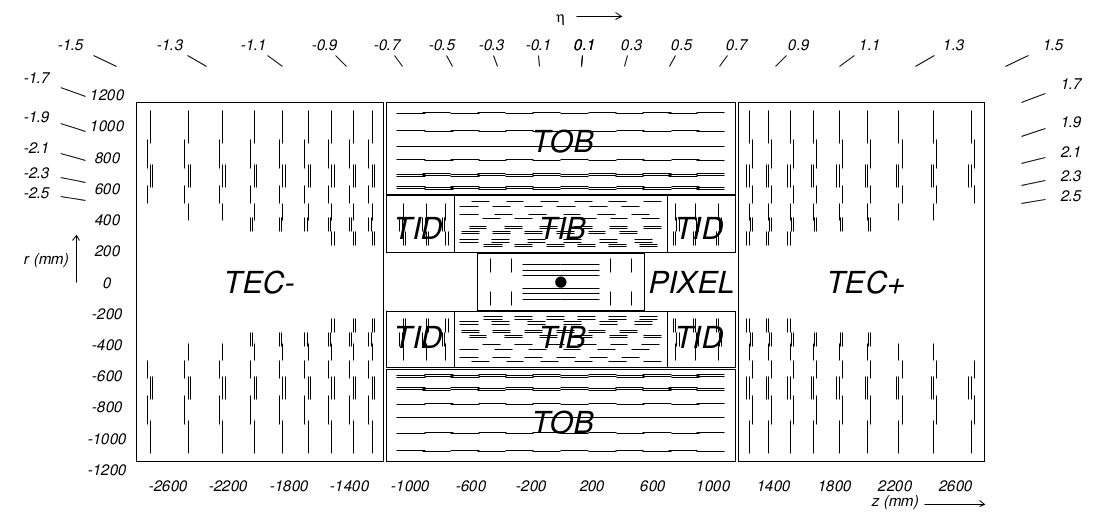
\includegraphics[scale=0.4]{Figures/TrackerLayout.png} \\
       \caption[The longitudinal cross section of the layout of the CMS tracker.]{The longitudinal cross section of the layout of the CMS tracker~\cite{CMSdetector}.  Each line represents a module, with double lines indicating back-to-back modules that deliver stereo hits.}
\label{figapp:TrackerLayout}
\end{figure}


\begin{figure}[!Hh]
       \centering
       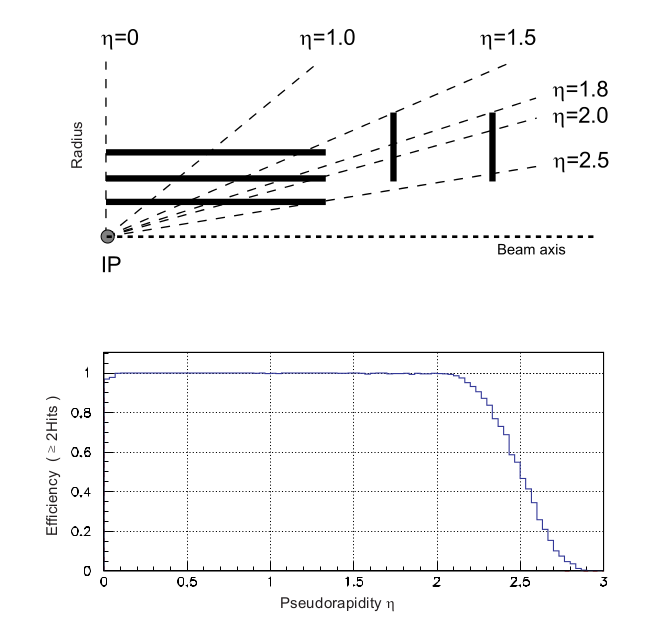
\includegraphics[scale=0.6]{Figures/PixelCoverage.png} \\
       \caption[The layout of the pixel detector.]{The geometrical layout of the pixel detector (top) and the hit coverage with respect to pseudorapidity (bottom)~\cite{CMSdetector}.}
\label{figapp:PixelCoverage}
\end{figure}


The other three systems compose the strip tracker and are located at radii from 20 cm to 116 cm.  The Tracker Inner Barrel and Inner Disks (TIB/TID) are composed of 4 barrel layers supplemented by 3 encdcap disks at each end, covering a radius up to 55 cm.  Thus the TIB/TID delivers up to 4 $r-\phi$ measurements per trajectory.  It uses 320 $\mu\text{m}$ thick silicon micro-strip sensors oriented parallel to the beam axis in the barrel and perpendicular to it in the endcaps.  The strip pitch (inter-strip distance) is 80 $\mu\text{m}$  on layers 1 and 2 and 120 $\mu\text{m}$ on layers 3 and 4 of the TIB, varying from 100 $\mu\text{m}$ to 141 $\mu\text{m}$  in the TID.  The strip pitch, width, and length are chosen to minimize inter-strip capacitance which in turn optimizes the resolution and occupancy as well as ensuring high voltage operational stability~\cite{STRIPtracker}.  The TIB/TID is in turn surrounded by the Tracker Outer Barrel (TOB) which consists of 6 barrel layers of 500 $\mu\text{m}$ thick sensors extending to a radius of 116 cm.  The strip pitches are 183 $\mu\text{m}$ on the first 4 layers and 122 $\mu\text{m}$ on the last 2 layers.  The TOB extends in $z$ between $\pm118$ cm and beyond it lie the Tracker EndCaps (TEC).  Each TEC consists of 9 disks covering $124\text{cm} < |z| < 282 \text{cm}$ and $22.5\text{cm} < |z| < 113.5\text{cm}$.  There are 4 inner rings with 320 $\mu\text{m}$ thick strips and 5 outer rings with 500 $\mu\text{m}$ thick strips, averaging pitches ranging from 97 $\mu\text{m}$ to 184 $\mu\text{m}$.  

In addition to the modules listed above, the first two layers and rings of the TIB, TID, and TOB as well as rings 1, 2, and 5 of the TECs contain a second micro-strip module mounted back-to-back with a stereo angle of 100 mrad which provides a measurement in the second coordinate ($z$ in the case of the barrel, $r$ in the case of the disks).  The strip tracker layout in total assures at least approximately 9 hits in the $|\eta| < 2.4$ range, 4 of which are two-dimensional measurements.  The complete coverage of the strip tracker ends at $|\eta| = 2.5$, the overall number of measurment points in the strip tracker is given as a function of $\eta$ in Figure~\ref{figapp:StripCoverage}.


\begin{figure}[!Hh]
       \centering
       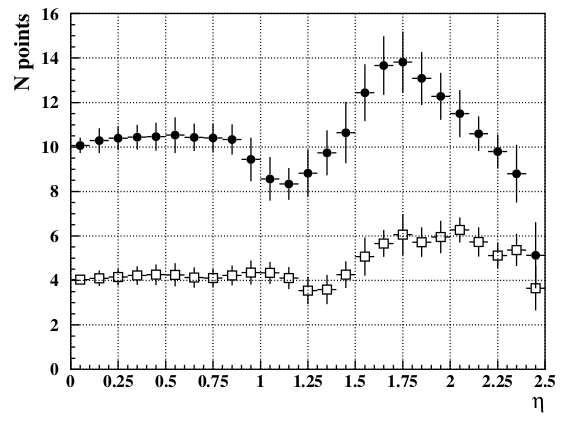
\includegraphics[scale=0.6]{Figures/StripCoverage.png} \\
       \caption[The coverage of the strip tracker.]{The number of measurment points in the strip tracker with respect to $\eta$, black circles represent the total number while white squares represent stereo layers~\cite{CMSdetector}.}
\label{figapp:StripCoverage}
\end{figure}


The pixel and strip detector modules performed very well in Run I (in 2011 and 2012), the hit efficiencies are shown in Figure~\ref{figapp:TrackerHitEfficiency}.  The tracker allows for accurate reconstruction of charged particle tracks as well as high-resolution measurements of the interaction vertices, which are both described in detail in Section~\ref{trackreco}.  


\begin{figure}[!Hh]
       \centering
       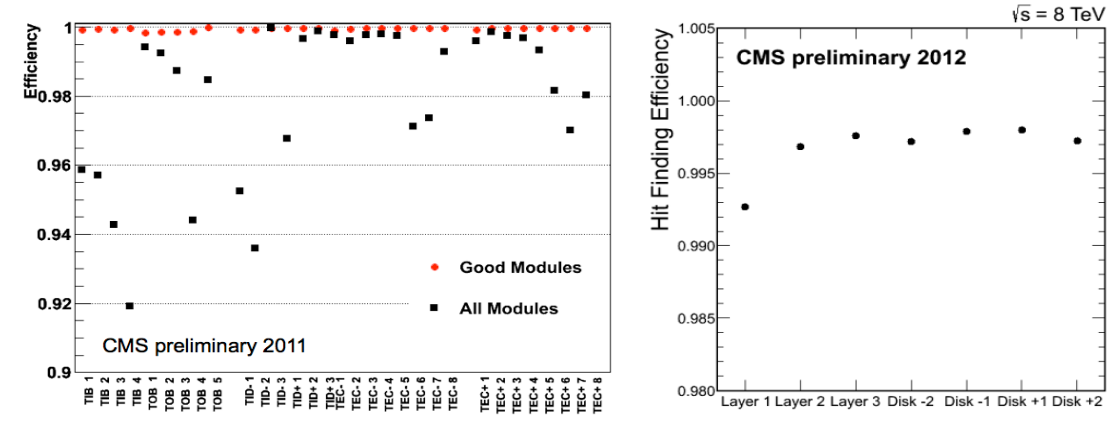
\includegraphics[scale=0.4]{Figures/TrackerHitEfficiency.png} \\
       \caption[The hit efficiency of the CMS tracker.]{The single hit efficiency of the strip (left) and pixel (right) trackers~\cite{STRIPtracker}.  Only the good (fully operational) modules were considered for the pixels.}
\label{figapp:TrackerHitEfficiency}
\end{figure}


\subsection{The Electromagnetic Calorimeter}
\label{ecal}

The electromagnetic calorimeter (ECAL) immediately surrounds the silicon tracker.  The ECAL is a hermetic and homogeneous calorimeter which is composed of 75,848 lead tungstate ($\text{PbWO}_4$) crystals in total, with 61,200 located in the central barrel section and 7,324 in each endcap.  A preshower detector is located in front of the endcap crystals, which serves to identify neutral pions in the endcaps and help electron identification against minimum ionizing particles~\cite{CMStdr}.  


The barrel portion of the ECAL (EB) covers a pseudorapidity range of $|\eta| < 1.479$ with an inner radius of 1.29 m.  The granularity is 360-fold in the $\phi$-direction, and (2$\times$85)-fold in $\eta$, resulting in the total of 61,200 individual crystals.  The crystals themselves are tapered in shape, slightly varying with position in $\eta$.  The endcap portion (EE) covers a pseudorapidity range of $1.479 < |\eta| < 3.0$, with a longitudinal distance from the inner surface to the interaction point of 315.4 cm.  The preshower detector (ES) sits directly in front of each EB, covering a pseudorapidity range of $1.653 < |\eta| < 2.6$. The overall layout of the ECAL is given in Figure~\ref{figapp:ECALlayout}.  




\begin{figure}[!Hh]
       \centering
       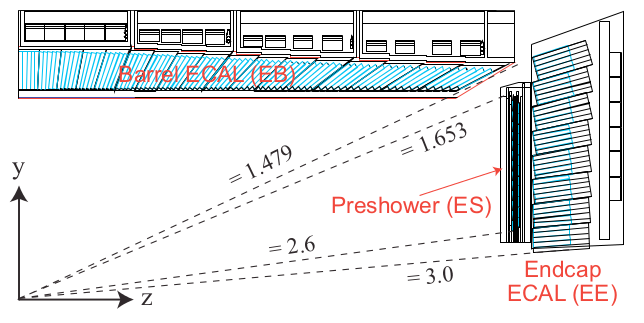
\includegraphics[scale=0.6]{Figures/ECALlayout.png} \\
       \caption[The layout of the CMS electromagnetic calorimeter.]{The layout of the ECAL, showing the Barrel ECAL (EB), Endcap ECAL (EE), and Preshower ECAL (ES)~\cite{CMStdr}.  The dashed lines are labeled with pseudorapidity values for reference.}
\label{figapp:ECALlayout}
\end{figure}


A driving criterion in the design of the ECAL was the ability to detect decays to two photons, a main decay mode of the Higgs boson.  The characteristics of the $\text{PbWO}_4$ crystals made them an appropriate choice to help meet this criterion.  The density (8.28 g/$\text{cm}^3$) and short radiation length of 0.89 cm (defined as the mean path length over which a relativistic particle loses energy by a factor of $1/e$) allows for a compact design.  The small Moli$\grave{\text{e}}$re radius of 2.2 cm (the radius of a cylinder transverse to a charged particle's direction of flight in which on average at least 90\% of the particle's energy is deposited) provides a fine granularity.  Additionally, in the years leading up to the construction of the LHC, $\text{PbWO}_4$ crystal production improved, becoming capable of producing optically clear and radiation-hard crystals.  The scintillation decay time of the $\text{PbWO}_4$ crystals in the ECAL is on the same order as the LHC design bunch crossing time, approximately 80\% of the light is emitted in 25 ns.  At the design operation temperature of $18^{\circ}$ C the light output is approximately 4.5 photoelectrons per MeV.  The scintillated light is blue-green in color, with a broad maximum wavelength of 420-430 nm~\cite{CMSdetector}.

The scintillated light is collected by photodetectors located at the end of each crystal.  In the barrel, avalanche photodiodes (APDs) that are specially produced for the CMS ECAL are used.  Two are placed on the backs of each crystal module.  In the endcap, the photodetectors used are vacuum phototriodes (VPTs), also specially produced for the ECAL, with one per crystal module.  ECAL modules of both the endcap and the barrel are shown with their attached photodetectors in Figure~\ref{figapp:ECALphotodetectors}.

\begin{figure}[!Hh]
       \centering
       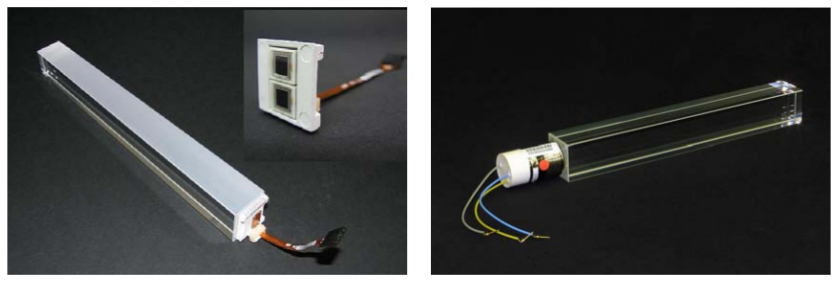
\includegraphics[scale=0.5]{Figures/ECALphotodetectors.png} \\
       \caption[Photodetectors and crystal modules in the CMS eletromagnetic calorimeter.]{$\text{PbWO}_4$ crystals with their photodetectors attached~\cite{CMStdr}.  A barrel crystal with attached APD (left), detached pair of APDs (left insert), and endcap crystal with VPT attached (right).}
\label{figapp:ECALphotodetectors}
\end{figure}

The APDs and VPTs are fast and radiation hard and are able to operate in a 4-T magnetic field.  The $\text{PbWO}_4$ crystals output a relatively small amount of light, so both photodetector types must have strong amplification.  The APDs operate at a gain of 50 and cover an active area of 25 $\text{mm}^2$.  The VPTs, of which there are only one per crystal, operate at a mean gain of 10.2 in a zero field and cover an active area of approximately 280 $\text{mm}^2$.  When the VPTs are placed in a strong axial magnetic field the response is slightly reduced, and there is a variation of response with the angle of the VPT axis with respect to the field.  The mean response in a 4-T field is typically at least 90\% of that in a zero magnetic field.  Both the APDs and VPTs were tested and screened to ensure reliable operation for 10 years under the high luminosity LHC conditions.



\subsection{The Hadronic Calorimeter}
\label{hcal}


The hadronic calorimeter (HCAL) is located directly outside of the ECAL and its role is to measure the energies of hadron jets and to help infer the missing transverse energy in an event that may result from neutrinos and/or exotic particles.  The HCAL is composed of 4 main components: the barrel (HB), the endcap (HE), the outer (HO), and the forward (HF) calorimeters.  Each subcomponent is a sampling calorimeter using the well known calorimetry strategy of tile and wavelength shifting fibers~\cite{CMSdetector}.  The layout of these subsystems are given in Figure~\ref{figapp:HCALlayout}.


\begin{figure}[!Hh]
%       \centering
       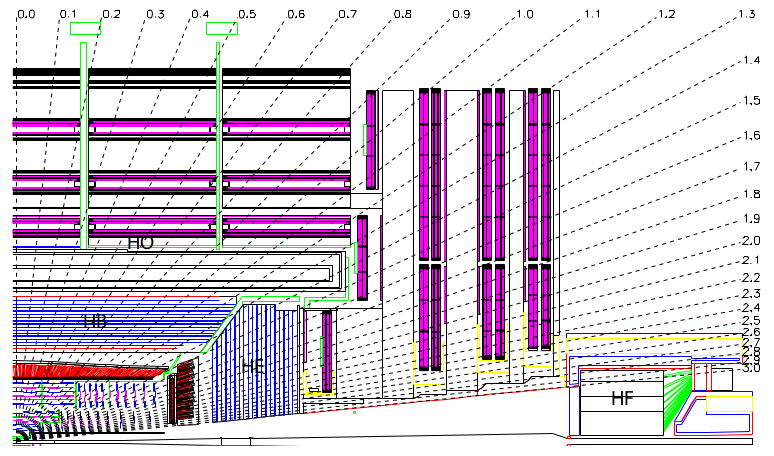
\includegraphics[scale=0.6]{Figures/HCALlayout.png} \\
       \caption[Layout of the CMS hadronic calorimeter.]{A longitudinal cross section of the layout of the CMS detector featuring the locations of the hadronic calorimeter: the barrel (HB), the endcap (HE), the outer HCAL (HO), and the forward HCAL (HF)~\cite{CMSdetector}.}
\label{figapp:HCALlayout}
\end{figure}

The HB inner radius is restricted by the outer edge of the ECAL, $R=1.77$ m, and the inner edge of the magnet coil, $R=2.95$ m.  It is composed of 36 identical azimuthal wedges which form each of two half barrels (HB+ and HB-), together covering the pseudorapidity range of $|\eta| < 1.3$.  Each wedge is is segmented azimuthally is segmented in to 4 sectors and is composed of brass absorber plates that are bolted together in a staggered fashion as to produce a configuration which contains no projective dead material for the full extent of the wedge.  For structural integrity the brass absorbers are reinforced by steel plates on the front and back of the wedges.  The scintillator, which is made of plastic, is divided into 16 $\eta$ sectors producing a segmentation of $(\Delta\eta,\Delta\phi) = (0.087, 0.087)$.  The light from the scintillators is brought out by wavelength shifting fibers and after exiting the scintillator the fibers are spliced to clear fibers.  These clear fibers bring the light to the hybrid photodiode for eventual data collecting.  

The HE cover a large portion of the pseudorapidity range, $1.3 < |\eta| < 3$, which is a region containing approximately 34\% of final state particles.  Because the HE is inserted into the end of a high T solenoidal magnet, the absorber had to be composed of a non-magnetic material.  In order to simultaneously satisfy that condition and others such as a maximum number of interaction lengths to contain hadronic showers, C26000 cartridge brass was used~\cite{CMSdetector}.  As with the HB, the HE absorbers are staggered to avoid creation of any projective dead material.  In addition, they are shaped to minimize any cracks between HB and HE, rather than being shaped to optimize single-particle energy resolution.  This is due to the fact that jet resolution in the HE is limited by pileup, magnetic effects, and parton fragmentation in any case.  Also as with the HB, the HE contain scintillators whose light is brought out via wavelenth shifting fibers to photodetectors and readout electronics.  

Between the electronic and hadronic barrel calorimeters (EB and HB) there is not enough stopping power in the central pseudorapidity region to provide adequate containment for hadronic showers.  Thus, to ensure that there is sufficent sampling depth for tha tregion, the HCAL is extended outside the solenoid with the HO, also called a tail catcher.  The HO uses the solenoid coil as an extra absorber and is used to identify showers that start late and to measure any additional shower energy deposited after the HB.  The HO is placed as the first sensitive layer in each of the five rings of the iron yoke (2.536 m wide along the z-axis).  It is segmented in to 12 identical azimuthal sectors, closely matching the geometry of the barrel muon system.  Together with the HE and the HB the HO is segmented in the $r,z$ plane according to Figure~\ref{figapp:HCALsegmentation}.  



\begin{figure}[!Hh]
%       \centering
       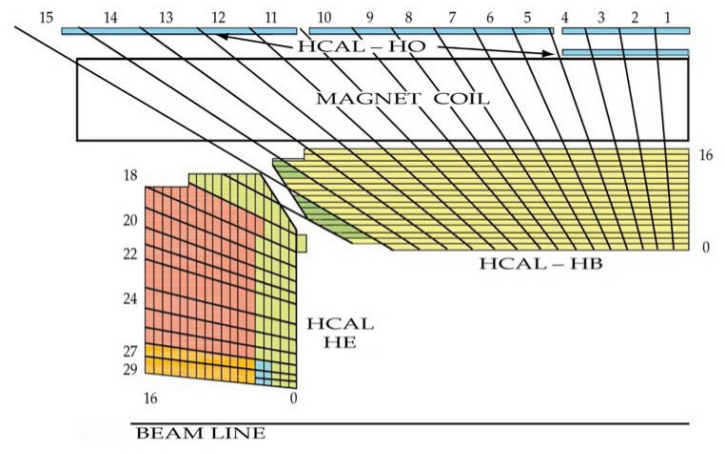
\includegraphics[scale=0.6]{Figures/HCALsegmentation.png} \\
       \caption[Segmentation of the CMS hadronic calorimeter.]{A cross section in the $r,z$ plane of the segmentation of the HB, HE, and HO~\cite{CMSdetector}.}
\label{figapp:HCALsegmentation}
\end{figure}

The HF is located in a region that experiences huge particle fluxes, the front face is located 11.2 m from the interaction point, with an inner radius of 12.5 cm and an outer radius of 130 cm.  It receives on average 760 GeV per proton-proton interaction as opposed to 100 GeV for the rest of the detector.  To cope with this environment the HF is housed in a hermetic radiation shield which consists of layers of 40 cm thick steel, 40 cm of concrete, and 5 cm of polyethylene.  Additionally, the active elements of the HF are radiation-hard quartz fibers.  The calorimeter itself is subdivided into two segments longitudinally, one which runs the full depth of the detector and one which only starts at a depth of 22 cm from the front,  which are read out separately.  This allows the HF to distinguish between showers generated by electrons and photons, which deposit a majority of their energy in the first 22 cm, from hadronic showers which deposit their energy roughly equally throughout the calorimeter.



\subsection{The Muon system}
\label{muons}

Precision measurement of muons is of critical importance, as many final state decays of exotic processes and signatures of supersymmetry include one or more muon muons, and the ``gold plated'' SM Higgs decay mode of $h \rightarrow ZZ \rightarrow 4 \mu$ (as well as a few other Higgs decay modes) produces many muons in its decay states.  Muon final states possess great discovery potential, as final states in which all leptons are muons are less affected by radiative losses in the tracker system.  Thus, as indicated by the experiment's middle initial, muon detection is a main role that the CMS detector must perform well.  The combined muon system has three functions: muon identification, momentum measurement, and triggering.  Good muon momentum resolutions and trigger capability are facilitated by the high-field solenoid magnet and the flux-return yoke.  The yoke also serves to absorb hadrons to assist with muon identification.

The muon system has the capability to reconstruct muon momentum and charge over the entire kinematic range of the LHC, and is composed of 3 separate types of gaseous particle detectors.  As with the calorimeters, the muon system is composed of a cylindrical barrel section and two planar endcap sections.  The eventual background rates the muon system was uncertain during construction, and the ability of the muon system to correctly measure the beam-crossing time at full LHC luminosity, so a dedicated trigger system was added in both the barrel and endcap sections.  This system, consisting of Resistive Plate Chambers (RPC) provides a fast and fully independent trigger with a sharp $p_T$ threshold over a large pseudorapidity range, $|\eta|< 1.6$.  In the barrel, where the overall muon rate and neutron-induced background is low, and the 4-T magnetic field is low as well, so drift chambers with rectangular drift cells are used.  This system, the Drift Tubes (DT), covers a pseudorapidity range of $|\eta| < 1.2$.  In the endcap regions the muon and background rates are high, and the magnetic field is large and non-uniform, so Cathode Strip Chambers (CSC) are used because of their fast response time, fine segmentation, and radation-hardness.  The CSCs cover a pseudorapidity range of $0.9 < |\eta| < 2.4$.  The layout of these three systems is shown in a quadrant cutout of the CMS detector shown in Figure~\ref{figapp:Muoncutout}.





\begin{figure}[!Hh]
%       \centering
       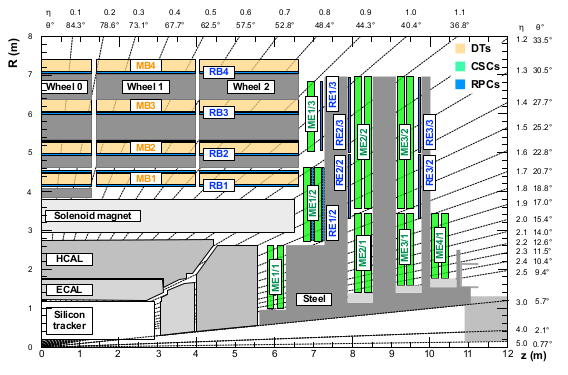
\includegraphics[scale=0.8]{Figures/Muoncutout.png} \\
       \caption[The layout of the CMS muon system.]{The cross section of a quadrant of the CMS detector, in the $R-z$ plane~\cite{CMSperformance}.  The muon systems are featured, the four DT stations (light orange) are labeled MB, the CSCs (green) are labeled ME, and the RPCs (blue) which are in both barrel and endcap are labeled both MB and ME, respectively.  MB stands for ``muon barrel'' and ME for ``muon endcap''.  The dark gray regions represent the steel disks.}
\label{figapp:Muoncutout}
\end{figure}


\subsubsection{The Resistive Plate Chamber system}
\label{rpcs}

The RPCs are gaseous parallel-plate detectors that provide a time resolution comparable to that of scintillators.  An RPC is capable of identifying the time of an ionising event in a significantly shorter time than the 25ns between two consective LHC bunch crossings.  A muon trigger based on RPCs can identify the bunch crossing to which a muon track is associated unambiguously, and thus the RPCs are a detector system dedicated to triggering.  The RPCs cover a pseudorapidity of $|\eta| < 1.6$ which covers the entire range of the DTs and a portion of the range of the CSCs.  

The RPCs are double-gap (called ``up'' and ``down'' gaps) gaseous detectors, operated in avalanch mode with common pick-up read-out strips located between the two gaps.  Each gap consists of a pair of 2 mm thick bakelite plates coated in a thin graphite layer encapsulating the gap which is filled by gas mixture of 95.2\% Freon, 4.5\% isobutane, and 0.3\% sulphur hexaflouride.  The plates are held to a voltage of 9.6 kV, and muons that traverse the gas ionize an atom in the gas, causing an avalanch which induces a charge that is readout by the on-board electronics.  

The RPCs are partioned in the $\eta$-direction, in two and three partitions (called rolls) in the barrel and endcap, respectively.  The layout of a typical barrel RPC is shown in Figure~\ref{figapp:RPClayout}.  The RPCs are arranged in stations following a similar sequence to the DTs and RPCs.  The RPC barrel (RB) has 4 stations, RB1-4, while the RPC endcap (RE) has 3 stations, RE1-3, totalling 480 chambers overall.  



\begin{figure}[!Hh]
%       \centering
       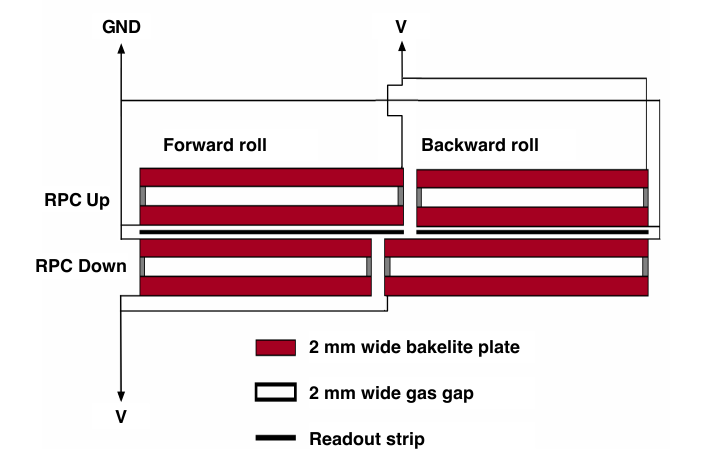
\includegraphics[scale=0.6]{Figures/RPClayout.png} \\
       \caption[The layout of a resistive plate chamber.]{A schematic of a barrel RPC with two partitions (rolls)~\cite{CMSperformance}.}
\label{figapp:RPClayout}
\end{figure}



\subsubsection{The Drift Tube system}
\label{dts}

The DTs are located in the barrel, covering a pseudorapidity range of $|\eta < 1.2|$.  In this region the muon rate is low, the neutron background is small (except for at the outermost layer of the DTs), and the magnetic field is predominantly uniform with a strength of 0.4 T and lower~\cite{CMSperformance}.  Thus drift chambers are used with rectangular cells and electrical field shaping implemented.  There are four stations in the barrel, labeled MB1-4, which are divided into 12 $\phi$-segments.  

The DTs contain basic elements called drift cells, with a transverse area of $42 \times 13 \text{mm}^2$ and a 50 $\mu$m diameter gold-plated anode wire at the center.  A voltage of 3600 V is applied to the wire, and 4 electrodes are used (including 2 cathode strips) to shape the drift field: 2 on the ground planes between layers and 2 on the side walls of the tube.  These electrodes are held at 1800 and -1200 V, respectively.  The layout of the drift cell with the drift paths and an example incident muon path is depicted in Figure~\ref{figapp:DTlayout}.



\begin{figure}[!Hh]
%       \centering
       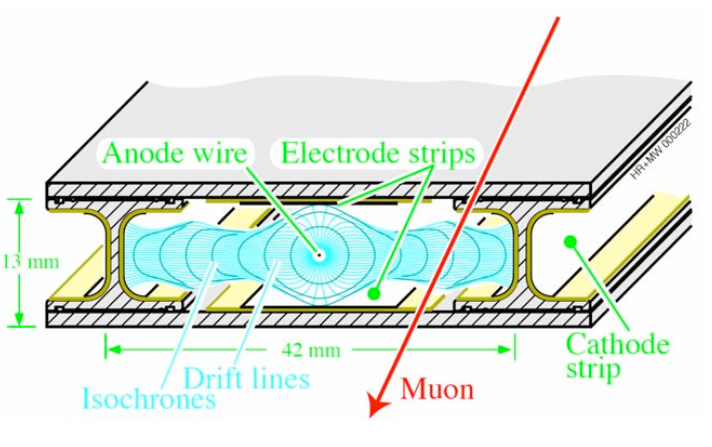
\includegraphics[scale=0.6]{Figures/DTlayout.png} \\
       \caption[The layout of drift cell of the drift tube system.]{A schematic of a drift cell, shown with the drift lines and an example incident muon path~\cite{CMSdetector}.}
\label{figapp:DTlayout}
\end{figure}

The gas mixture which is ionized by incident muons is an 85\%/15\% blend of argon (Ar) and carbon dioxide (CO$_2$).  This provides good quenching properties, as well as a saturated drift velocity of approximately 55 $\mu$m/ns and a maximum drift time of 400 ns.  These drift cells are staggered, with four layers of parallel cells forming a superlayer (SL).  Each DT chamber consists of 2 SLs that measure the $r-\phi$ coordinates and one orthogonal SL that measures the $r-z$ coordinate (except for the outermost layer of DTs, MB4, which only has an $r-\phi$ layer).  



\subsubsection{The Cathode Strip Chamber system}
\label{cscs}



The CSCs cover a pseudorapidity range of $1.2 < |\eta| < 2.4$, and consist of a total of 473 chambers in the first LHC run.  There are 108 in the first station (ME1), 54 in the second and third (ME2 and ME3), and 18 in the inner ring of the outermost station (ME4), as depicted in Figure~\ref{figapp:Muoncutout}.  On one side of the CMS detector, 5 CSCs were placed in an outer ring on the 4th station (ME4/2), and these were expanded to the full 18 per endcap in the second LHC run.  

CSCs are trapezoidal in shape and cover either $10^\circ$ or $20^\circ$ in $\phi$.  All except for ME1/3 overlap and provide continuous $\phi$-coverage.  They aare comprised of 6 anode wire planes interspersed with 7 cathode panels.  The wires run azimuthally and define the radial coordinate of a track.  The strips are milled directly on to the cathode panels and run lengthwise at a constant width in $\Delta\phi$.  While there are varying total sizes of chambers, the largest ones (ME2/2 and ME3/2) are approximately $3.4 \times 1.5 \text{ m}^2$ in size, and a sample schematic layout of a typical CSC is given in Figure~\ref{figapp:CSClayout}.




\begin{figure}[!Hh]
       \centering
       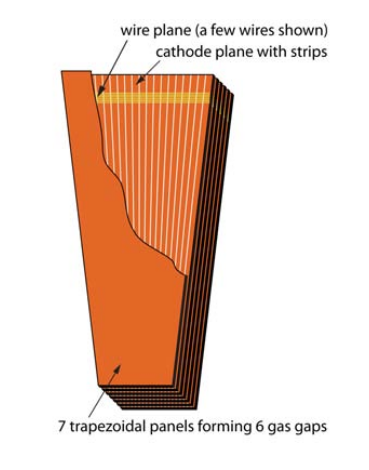
\includegraphics[scale=0.8]{Figures/CSClayout.png} \\
       \caption[The layout of a cathode strip chamber.]{A schematic of a CSC, shown with all six layers~\cite{CMSdetector}.}
\label{figapp:CSClayout}
\end{figure}



The nominal gas mixture used in the CSCs for ionization is 40\% Ar, 50\% $\text{CO}_2$, and 10\% $\text{CF}_4$.  The primary role of the $\text{CO}_2$ is as a non-flammable quencher for achieving large gas gains, and the role of the $\text{CF}_4$ is to prevent polymerization on the anode wires.  The nominal operating voltage was chosen to be 3.6kV which corresponds to a gas gain on the order of $7 \times 10^4$, except for the inner stations (ME1), for which 3.3kV was chosen.  These voltages provide very high efficiencies with an adequate signal-to-noise ratio.  

Each chamber has a set of anode front end boards (AFEBs) that are amplifier-discriminators and serve to initially shape and read out charge avalanches from incident muons ionizing the gas.  All the AFEBs send their output to an FPGA-based anode local charged track (ALCT) board, of which there is one per chamber.  The ALCT checks every bunch crossing for patterns in the 6 planes that are consisent with a muon track originating from the interaction point.  Any pattern that is found is called an ALCT, and serves as a trigger primitive that is transferred downstream for further decisions on whether the event should be recorded as data.  A depiction of this avalanche and ALCT formation is given in Figure~\ref{figapp:CSCavalanche}.


\begin{figure}[!Hh]
       \centering
       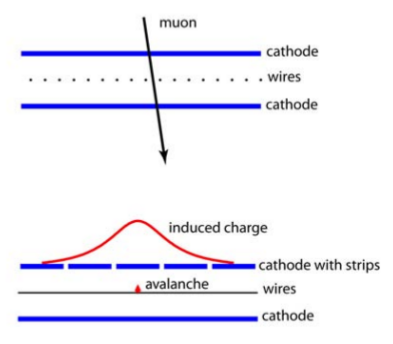
\includegraphics[scale=0.5]{Figures/CSCavalanche.png}
       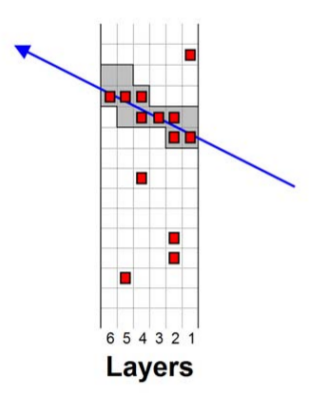
\includegraphics[scale=0.5]{Figures/CSCalct.png} \\
       \caption[A schematic depiction of an avalanche in a cathode strip chamber and an anode local charged track.]{A schematic view of one gap, depicting the principle of CSC operation (right).  The charge induced on the cathode strips is interpolatd, and a localization of the avalanche along the direction of the wire is found.  A pattern of these hits is quickly matched to form an anode local charged track (ALCT, right)~\cite{CMSdetector}.}
\label{figapp:CSCavalanche}
\end{figure}

Each CSC has 5 cathode front end boards (CFEBs) that serve to manage the charge deposited on the cathode strips.  The CFEBs contain more logic than the AFEBs, and use a comparator network that uses on board amplifier shaper outputs to achieve a resolution corresponding to each half strip.  This is achived via a comparison for every group of 3 adjacent strips, determining the amplitude of the central strip signal and comparing it to the central-to-left and central-to-right signal.  Thus if the charge on the central strip is above the threshold, and the charge on the right strip is larger than on the left, the hit position must be in the right half of the central strip.  This is depicted in Figure~\ref{figapp:CSCclct}.

\begin{figure}[!Hh]
       \centering
       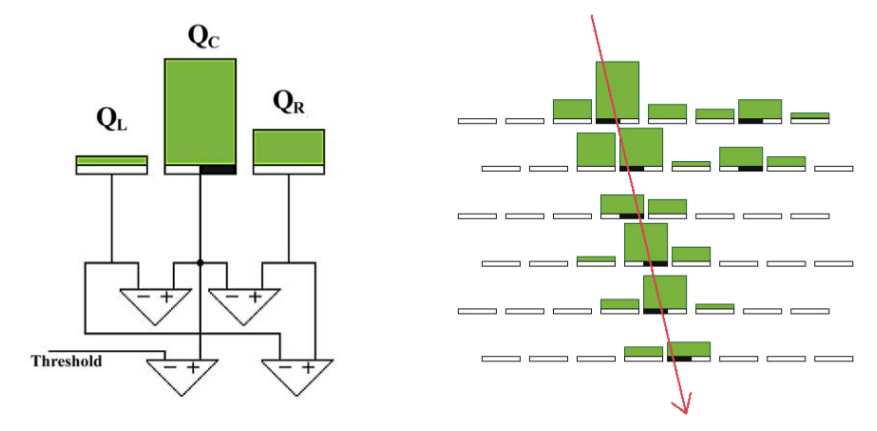
\includegraphics[scale=0.5]{Figures/CSCclct.png} \\
       \caption[A schematic depiction of the formation of a cathode local charged track.]{A schematic depiction of the CFEB comparator network (left) and how half-strip resolution is acheived.  A muon track is depicted in red (right) and the white rectangles represent cathode strips.  Each half-strip where a hit is found is colored black, and the green rectangles represent the amplitude of the signal, showing how the comparator network makes the half-strip decisions~\cite{CMSdetector}.}
\label{figapp:CSCclct}
\end{figure}

The half-strip cathode local charged track hits and the anode local charged track hits are both sent to a piece of off-chamber electronics called the trigger motherboard (TMB).  There is one TMB per chamber, and each can create two 2-dimensional LCTs from the ALCT and CLCT that it receives from the chamber.  These 2D LCTs are sent on to muon port cards (MPCs), each of which collects hits from 9 chambers.  The MPC collects the 2D LCTs, sorts them, and finds the 3 highest quality candidates to send further upstream to the Level-1 muon trigger electronics.  This path is shown in Figure~\ref{figapp:CSCreadout}.

The raw data is collected by the data acquisition, or DAQ, motherboards (DMBs).  They are also located off-chamber, in peripheral crates, with the TMBs and MPC, and there is one per chamber.  The data passed to the DMBs consist of anode and cathode comparator hits in a time window that is up to 32 bunch crossings long.  These data that are collected by the DMB are in turn passed on to the detector dependent unit (DDU) and then to a data concentration card (DCC) and then finally on to the CMS filter farm in order to be processed by the CMS high level trigger (HLT) software.  The approximate event size per chamber is 4-5 kBytes.  These electronics are also shown in Figure~\ref{figapp:CSCreadout}.

If the Level-1 trigger accepts the data from a collision (this decision being made by Level-1 electronics from all subsystems), a ``Level 1 accept'', or L1A, is sent back out.  This signal, as well as the LHC clock and all other control signals, is distributed to all the CSC electronics by the clock control board (CCB).  This is also shown in Figure~\ref{figapp:CSCreadout}.  The raw anode and cathode local charged track data is only sent upstream in coincidence with an L1A signal, so the CSC read-out system is intrinsically zero-suppressed.  

\begin{figure}[!Hh]
%       \centering
       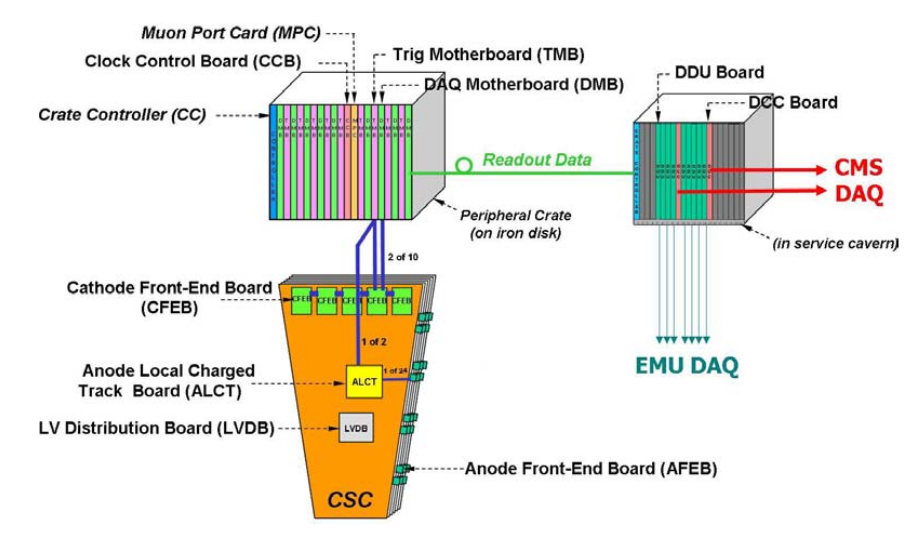
\includegraphics[scale=0.5]{Figures/CSCreadout.png} \\
       \caption[A schematic of the cathode strip chamber electronic trigger and readout system.]{The schematic layout of the cathode strip chamber trigger and read-out electronics~\cite{CMSdetector}.}
\label{figapp:CSCreadout}
\end{figure}


Something about ODMB?



\subsection{The Trigger system}
\label{trigger}


The LHC delivers collisions to the CMS detector at a beam crossing interval of 25ns (or 50ns in 2011 and 2012), corresponding to a crossing frequency of 40 MHz at design parameters.  At this design frequency, and at nominal instantaneous luminosity, an average of 20 collisions per crossing will occur.  As it is impossible to store and process data for some many events, a drastic reduction in the rate of event storage is necessary.  This necessary reduction is performed by the trigger system, which is the the beginning of the physics event selection process.  

The procedure of performing this reduction in rate is separated in to two steps, and thus two systems.  The first is the Level-1 Trigger system (L1 Trigger) and it is composed of custom-designed, mostly programmable electronics.  The second is the High-Level Trigger (HLT), which is a software-based system implemented in a filter farm of approximately one thousand commercial processors.  Combined, the L1 Trigger and HLT effect a rate reduction of at least a factor of $10^6$.  



\subsubsection{The L1 Trigger}
\label{l1trigger}

The design output rate of the L1 Trigger is 100 kHz, which in practice is limited to 30 kHz, with an approximate safety factor of three.  The L1 Trigger uses relatively coarsely segmented data from the calorimeters and the muon system, while keeping the high-resolution data in pipelines in the front-end subdetector electronics.  In order to ensure flexibility, the hardware for the L1 Trigger is implemented in FPGA (Field Programmable Gate Array) technology in most places, but some ASICs and memory lookup tables (LUTs) are also used where speed and radiation resistance is important.  

The L1 Trigger is split in to local, regional, and global components.  At the bottom end, ``closest'' to the subdetectors themselves, the local component called Trigger Primitive Generators (TPGs) are based on energy deposits in the calorimeters and track segments or hit patterns in the muon chambers.  These TPGs are passed to the Regional Triggers which combine their information and use logic to rank and sort trigger objects such as electron or muon candidates in regions limited spatially.  The ranking is determined as a function of energy or momentum and quality, which reflects the confidence in the L1 measurements which is in turn based on the subdetector properties, electronics, and the information available.  The Global Calorimeter and Muon triggers determine the best-quality calorimeter and muon objects across the entire CMS detector and transfer those candidates to the Global Trigger.  The Global Trigger, finally, takes the decision to reject an event or to accept it for further decision making by the HLT.  This decision is based both on algorithmic calculations with the candidate objects and on the readiness of the subdetectors and the data acquisition system (DAQ), and is sent back to the subdetectors via the L1 Accept signal (L1A).  The overall architecture of the L1 Trigger system is shown in Figure~\ref{figapp:L1Tarchitecture}.  

\begin{figure}[!Hh]
%       \centering
       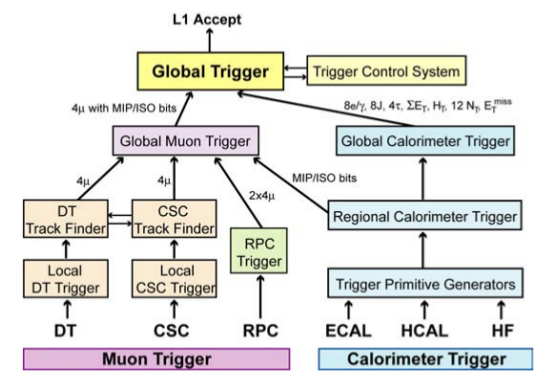
\includegraphics[scale=0.7]{Figures/L1Tarchitecture.png} \\
       \caption[Architecture of the Level-1 Trigger.]{The architecture of the L1 Trigger~\cite{CMSdetector}.  The trigger layers are shown with what information is sent to the Global Trigger: Muons ($\mu$), minimum-ionizing particle and isolation bits (MIP/ISO), electrons and photons ($e/\gamma$), jets (J), taus ($\tau$), total transverse energy ($\Sigma \text{E}_\text{T}$), total hadronic transverse energy($\text{H}_\text{T}$), number of jets passing various transverse energy requirements ($\text{N}_\text{T}$), and missing transverse energy ($\text{E}^\text{miss}_\text{T}$).}
\label{figapp:L1Tarchitecture}
\end{figure}

The TPGs in the Calorimeter Trigger subdivide both calorimeters in to trigger towers.  The TPGs compute the sums of transverse energies measured in the ECAL crystals or HCAL read-out towers in order to obtain the entire trigger tower $\text{E}_T$  and determine the correct bunch crossing.  The TPGs then are transmitted to the Regional Calorimeter Trigger (RCT) which is responsible for multiple tasks.  The RCT determines regional candidates for electrons and photons via determining the tower with the largest energy deposit and then applying two shower profile requirements: a fine-grained crystal energy profile that reflects teh lateral shape of a shower, and a requirement based on the ratio of deposited energies in the hadronic and electromagnetic portions.  It also requires there be at least one quiet corner in one of the course sections surrounding the hit.  This strategy is depicted in Figure~\ref{figapp:CALtrigger}.  The RCT also sums transverse energies in the calorimeters, determines $\tau$-veto bits based on the narrower shape of $\tau$ decays, and produces information relevant for muons in the form of minimum-ionizing particle (MIP) and isolation (ISO) bits.  Finally, the Global Calorimeter Trigger (GCT) determines the jets, total transverse energy and missing transverse energy, jet counts, and the jet-only transverse energy sum given a programmable threshold ($\text{H}_T$).  

\begin{figure}[!Hh]
%       \centering
       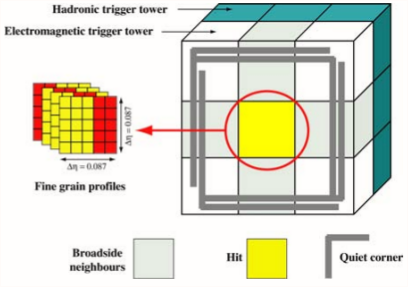
\includegraphics[scale=0.6]{Figures/CALtrigger.png} \\
       \caption[Electron/photon trigger strategy.]{The algorithm the RCT uses for electron/photon triggering~\cite{CMSdetector}.}
\label{figapp:CALtrigger}
\end{figure}

The TPGs in the muon trigger are sourced from all three muons subsystems.  The CSCs in the endcap deliver 3-dimensional track segments (straight line segments, LCTs).  The DTs likewise contribute track segments, which are track segments in the $\phi$-projection and hit pattterns in the $\eta$-projection.  All chambers also identify the bunch crossing from which the event originated from.  The regional muon trigger is based on the DT and CSC Track Finders (DTTF, CSCTF), which serve to create tracks out of the individual segments they receive and thus identify muon candidates along with their transverse momenta, locations, and quality.  The functionality of both the DTTF and CSCTF fits into high-density FPGAs: DTTF segmentation in the central wheel is $2 \times 12$ half-width sectors and in the four outer wheels it is 12 full-width sectors each, while the CSCTF segmentation is by $2 \times 6$ $60^\circ$-sectors.  The CSCTF synchronizes the data and uses extrapolation to form an overall track.  Then the $p_T$ is assigned via lookup tables based on the $\phi$-information from three stations.  The overall strategy for the DTTF is the same, which also uses some pattern matching in the $\eta$ coordinate.  This algorithm is depicted, for the DTTF, in Figure~\ref{figapp:TrackFinder}.  The Global Muon Trigger (GMT) is fed the muon candidates from the DTTF, CSTF, and RPC Trigger and uses them to reduce repeat muon measurements vai merging kinematic parameters and canceling duplicates.  Muons are also back extrapolated to the vertex using the MIP/ISO bits from the calorimeters which are in turn also added to the GMT output.  Finally, the muons are sorted by transverse momentum and quality, to create four candidates to be given to the Global Trigger.

\begin{figure}[!Hh]
       \centering
       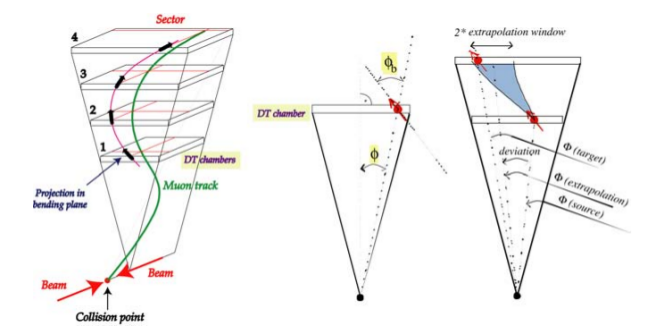
\includegraphics[scale=0.6]{Figures/TrackFinder.png} \\
       \caption[Track Finder track creation scheme.]{The algorithm the DTTF uses for muon candidate track extrapolation~\cite{CMSdetector}.  The CSCTF uses a very similar scheme, with 3-dimensional segments.}
\label{figapp:TrackFinder}
\end{figure}

The Global Trigger (GT) takes the decision to accept or reject an event at Level-1 based on the trigger objects that are delivered to it from the GCT and GMT.  The algorithms vary in complexity, with the most basic ones consisting of applying $p_T$ or $E_T$ thresholds to a single object, or requiring minimum jet multiplicities.  Location and quality information is available as well, so more complex algorithms taking into account event topology cand be programmed.  Up to 128 algorithms can be executed in paralle, and for normal physics data this single trigger mask is applied, with the L1A decision being taken accordingly.  



\subsubsection{The HLT}
\label{hlt}

Unlike the L1 Trigger, the HLT operates on software.  It serves to further reduce the output rate of the L1 Trigger of approximately 30 MHz to 100 Hz.  It consists of a variety of trigger paths based on object kinematics and quality criteria.  However, since it has access to the complete data read-out, it is capable of performing more complex calculations similar to those used by off-line analysis software.  Its goal is to both reduce rate and ensure that events saved match the interest of physics studies, so events are partially reconstructed even in the cases of simple kinematics-based criteria.  HLT algorithms evolve with experience, optimizing the usefullness for off-line analysis.  Additionally, in 2011 and 2012, the instantaneous luminosity delivered by the LHC increased continuosly, so some HLT trigger paths evolved with time to compensate for this and maintain a relatively constant rate of 100 Hz throughout the run periods.  Some HLT triggers also ``prescaled'' events, only saving a sampling of events (saving a $1/N$ fraction of events, where $N$ is called a prescale) that would otherwise increase the rate by large quantities, these prescales were also varied throughout run periods.
